
\documentclass[11pt]{article}
\usepackage{fullpage}
\usepackage{siunitx}
\usepackage{hyperref,graphicx,booktabs,dcolumn}
\usepackage{stata}
\usepackage[x11names]{xcolor}
\bibliographystyle{unsrt}
\usepackage{natbib}
\usepackage{pdflscape}


\usepackage{chngcntr}
\counterwithin{figure}{section}
\counterwithin{table}{section}

\usepackage{multirow}
\usepackage{booktabs}

\newcommand{\specialcell}[2][c]{%
  \begin{tabular}[#1]{@{}c@{}}#2\end{tabular}}
\newcommand{\thedate}{\today}

\usepackage{pgfplotstable}

\bibliographystyle{unsrt}
\renewcommand{\bibsection}{}
\makeatletter
\renewcommand\@biblabel[1]{	#1.}
\makeatother

\begin{document}


\begin{titlepage}
    \begin{flushright}
        \Huge
        \textbf{Identifying episodes of care in hospital admissions data for measures of disease burden: A protocol for individual-level data analysis}
\color{black}
\rule{16cm}{2mm} \\
\Large
\color{black}
\thedate \\
\color{blue}
https://github.com/jimb0w/HA \\
\color{black}
       \vfill
    \end{flushright}
        \Large

\noindent
Jedidiah I Morton, 
Adam Livori, 
Lee Nedkoff, 
Dianna J Magliano, 
Derrick Lopez,
Ingrid Stacey,
Zanfina Ademi.  \\

 
\noindent Correspondence to: \\
 \\
Jedidiah Morton \\
\color{blue}
\href{mailto:Jedidiah.Morton@Monash.edu}{Jedidiah.Morton@monash.edu} \\ 
\color{black}
Monash University, Melbourne, Australia \\
Baker Heart and Diabetes Institute, Melbourne, Australia \\\
 \\
\noindent
Adam Livori \\
\color{blue}
\href{mailto:adam.livori@gh.org.au}{adam.livori@gh.org.au} \\ 
\color{black}
Grampians Health, Ballarat, Australia \\
Monash University, Melbourne, Australia \\\
\normalsize
\end{titlepage}

\clearpage
\tableofcontents


\clearpage
\section{Introduction}
\label{introduction}

After cleaning hospital data for the \emph{nth} time on a new, 
completely different dataset from another country that required almost exactly
the same data processing as Australian admissions data, we decided
that it would be useful to have a standard protocol for processing hospital admissions data and 
defining episodes of care. 
This is supposed to be that protocol, although we welcome criticism and change -- 
this won't be perfect and all the nuances may not be covered, but this should serve as a good 
starting point for people attempting to analyse hospital data for the first time. 

This protocol will therefore outline most of the general principles for processing hospital admissions data
to define an episode of care, such as:
\begin{itemize}
\item Defining your event
\item Finding and removing ``duplicate'' admissions while keeping the information they contain
\item Finding and removing ``nested'' admissions while keeping the information they contain
\item Tagging and removing transfers
\end{itemize}

And will include a full worked example at the end. 
Some of this may be basic, but unless it's standardised, we (the research community) 
risk doing it incorrectly or different each time, 
or even just wasting time re-writing code every time 
(especially as a lot of this work is done by students new to this data). 

Finally, because we want to show individual-level data, we are going to use 
completely synthetic datasets for the first
part of this protocol,
but with cases based on common aspects of the data we have come across. 
In the synthetic dataset, we will assume the following variables are present:
\begin{itemize}
\item Unique inidividual identifier (\emph{id})
\item Admission date (\emph{admdate})
\item Separation date  (\emph{sepdate})
\item Diagnosis codes (\emph{diagx})
\item Admission source (\emph{admmode})
\item Separation destination (\emph{sepmode})
\end{itemize}

Therefore, the first part of this protocol (\ref{P1}) will go through worked examples
of how to process admissions data and define an episode of care. 
Then, in the second part of the protocol (\ref{P2}), we show a full example
using hospital episode statistics from inpatient data (the HESIN dataset) derived via 
linkage to the UK Biobank study that we have used for research previously (e.g., 
\color{blue} \color{blue}
\href{https://www.valueinhealthjournal.com/article/S1098-3015(24)02791-8/fulltext}{Morton et al., Value in Health, 2024}\color{black}).


\clearpage
\section{Defining an episode of care}
\label{P1}
\subsection{Data harmonisation and checks}

We have decided not to go through this in any detail, given that the specifics
will depend on the dataset in question. However, three brief comments
about data harmonisation and checks. First, check \emph{every} variable you use and create. 
As in, look at it, tabulate or histogram it, make sure it makes sense, check how
many missing values there are, and make sure
it makes sense in the context of other variables (e.g., is separation date
ever earlier than admission date?). Second, watch everything you do across
multiple examples, it is labourious, but worth it -- slow is smooth and smooth is fast
(i.e., it's much quicker to get it right the first time and then move on 
than to have to keep coming back to code you wrote a while ago every time you notice a 
new mistake/problem further along in the analysis). Third,
do not waste time perfecting code for 0.001\% of the dataset. The processes
and steps we outline below will work for most cases. We are also sure that these steps will miss things, 
but we are fairly confident those will be irrelevant -- usually you will be working with samples
that have at least 10,000 people in them, so having a handful of admissions coded incorrectly should
not impact analyses and we do not recommend scouring through
thousands of admissions to try and find them (especially if you are doing data checks, as recommended in our 
first comment, which will pick up any serious problems and you can then deal with them
individually if they are likely to impact your analysis).

\subsection{Defining admissions of interest}

After preparaing the variables you intend to use, 
the first step in defining an episode of care is
to define the event of interest. 
Defining an event or an admission you're interested in is 
primarily a clinical question and related to the study at hand. 
There are two common ways to define an event or admission, that we will now outline. 

First, using only the primary diagnosis for an admission. 
In this example, let's assume you're looking at myocardial infarctions (ICD-10 code: I21),
in which case, an event is probably only relevant when it's the primary diagnosis for an admission
(as when it's a secondary diagnosis it probably relates to a prior myocardial infarction
rather than an event). 
Usually, the first diagnosis code in a dataset is the primary reason for admission, so we will only
use that variable to tag all admissions for myocardial infarction. 

\color{Blue4}
\begin{stlog}. list in 1/10, separator(0)
{\smallskip}
     {\TLC}\HLI{7}{\TRC}
     {\VBAR} diag1 {\VBAR}
     {\LFTT}\HLI{7}{\RGTT}
  1. {\VBAR}  K833 {\VBAR}
  2. {\VBAR}  J749 {\VBAR}
  3. {\VBAR}  B895 {\VBAR}
  4. {\VBAR}  D209 {\VBAR}
  5. {\VBAR}  X408 {\VBAR}
  6. {\VBAR}  T700 {\VBAR}
  7. {\VBAR}  M308 {\VBAR}
  8. {\VBAR}  F421 {\VBAR}
  9. {\VBAR}  N609 {\VBAR}
 10. {\VBAR}  U688 {\VBAR}
     {\BLC}\HLI{7}{\BRC}
{\smallskip}
. *Our dataset is just randomly generated ICD-10 codes
. gen MI = 1 if substr(diag,1,3)=="I21"
(99,960 missing values generated)
{\smallskip}
. sort MI
{\smallskip}
. list in 35/44, separator(0)
{\smallskip}
     {\TLC}\HLI{12}{\TRC}
     {\VBAR} diag1   MI {\VBAR}
     {\LFTT}\HLI{12}{\RGTT}
 35. {\VBAR}  I211    1 {\VBAR}
 36. {\VBAR}  I219    1 {\VBAR}
 37. {\VBAR}  I216    1 {\VBAR}
 38. {\VBAR}  I215    1 {\VBAR}
 39. {\VBAR}  I219    1 {\VBAR}
 40. {\VBAR}  I210    1 {\VBAR}
 41. {\VBAR}  D729    . {\VBAR}
 42. {\VBAR}  J493    . {\VBAR}
 43. {\VBAR}  M742    . {\VBAR}
 44. {\VBAR}  C878    . {\VBAR}
     {\BLC}\HLI{12}{\BRC}
{\smallskip}
. *We successfully tag all admissions with a primary diagnosis for MI
\end{stlog}
\color{black}

The second way an event is often defined is 
when the position of the diagnosis (or procedure), is not relevant for the study. 
For this example, let's assume you're interested in 
diabetes status for an individual (ICD-10 codes: E10-E14),
and that there are 10 diagnoses associated with each admission. 

\color{Blue4}
\begin{stlog}. list in 1/10, separator(0)
{\smallskip}
     {\TLC}\HLI{80}{\TRC}
     {\VBAR} diag1   diag2   diag3   diag4   diag5   diag6   diag7   diag8   diag9   diag10 {\VBAR}
     {\LFTT}\HLI{80}{\RGTT}
  1. {\VBAR}  F609    O466    S516    V186    J121    G993    F631    L768    Y330     R266 {\VBAR}
  2. {\VBAR}  W790    O263    R353    F456    R119    F380    F081    K963    Z584     H879 {\VBAR}
  3. {\VBAR}  A433    S762    C249    O166    U852    N334    P040    R127    W641     V687 {\VBAR}
  4. {\VBAR}  H678    P884    I903    B003    H713    V166    L178    M872    H091     T575 {\VBAR}
  5. {\VBAR}  Y334    Z135    L002    K111    I956    U035    H706    W761    D399     U715 {\VBAR}
  6. {\VBAR}  N574    C216    M566    Q240    S958    W024    B033    A222    C830     S202 {\VBAR}
  7. {\VBAR}  J413    U880    B076    K921    E117    P650    V910    M413    D493     N804 {\VBAR}
  8. {\VBAR}  J280    H261    W341    E273    Z854    W896    F527    O826    B651     A676 {\VBAR}
  9. {\VBAR}  Z774    C835    P681    M020    U289    S419    Y873    R719    Y319     Q046 {\VBAR}
 10. {\VBAR}  R536    M761    K485    U037    Q858    D389    K805    Y912    A562     N392 {\VBAR}
     {\BLC}\HLI{80}{\BRC}
{\smallskip}
. *Our dataset is again just randomly generated ICD-10 codes
. gen DM = .
(1,000 missing values generated)
{\smallskip}
. forval i = 1/10 {\lbr}
  2. replace DM = 1 if inrange(diag`i',"E10","E149")
  3. {\rbr}
(0 real changes made)
(0 real changes made)
(3 real changes made)
(2 real changes made)
(2 real changes made)
(1 real change made)
(0 real changes made)
(1 real change made)
(1 real change made)
(3 real changes made)
{\smallskip}
. sort DM
{\smallskip}
. list in 9/18, separator(0)
{\smallskip}
     {\TLC}\HLI{85}{\TRC}
     {\VBAR} diag1   diag2   diag3   diag4   diag5   diag6   diag7   diag8   diag9   diag10   DM {\VBAR}
     {\LFTT}\HLI{85}{\RGTT}
  9. {\VBAR}  T185    B141    Y514    G173    X454    V472    S946    U199    E124     U983    1 {\VBAR}
 10. {\VBAR}  I130    U544    E110    Q410    H625    P330    Z654    M966    F785     L129    1 {\VBAR}
 11. {\VBAR}  F075    O516    O893    E108    J328    L046    H240    M068    O222     K244    1 {\VBAR}
 12. {\VBAR}  R051    A024    E146    E695    W157    V024    W073    V732    R030     S727    1 {\VBAR}
 13. {\VBAR}  D819    V569    N497    O920    E146    M240    Z526    E620    S187     Z155    1 {\VBAR}
 14. {\VBAR}  C788    Z222    V240    X218    L344    C379    X730    G937    A910     K515    . {\VBAR}
 15. {\VBAR}  C572    K222    L791    N781    N947    B416    J282    F679    S873     K855    . {\VBAR}
 16. {\VBAR}  L002    U164    K161    P976    X711    S121    C405    Q824    J102     O944    . {\VBAR}
 17. {\VBAR}  Z327    W346    I011    W123    K464    Q703    B714    K106    T648     U445    . {\VBAR}
 18. {\VBAR}  U084    N623    N170    Y053    V058    Y217    Z321    S776    N004     T339    . {\VBAR}
     {\BLC}\HLI{85}{\BRC}
{\smallskip}
. *We successfully tag all admissions with a diagnosis of diabetes at any position
\end{stlog}
\color{black}

The next step after defining the event
is usually to capture all admissions for individuals
with that event in your dataset (this just makes the dataset
smaller and thus faster and easier to work with). You
will see below why we need to keep all admissions for the individual, and not 
just those with the event of interest. 

\color{Blue4}
\begin{stlog}. sort id diag1
{\smallskip}
. list id DM if id == 5 | id == 6, separator(0)
{\smallskip}
      {\TLC}\HLI{9}{\TRC}
      {\VBAR} id   DM {\VBAR}
      {\LFTT}\HLI{9}{\RGTT}
  39. {\VBAR}  5    . {\VBAR}
  40. {\VBAR}  5    . {\VBAR}
  41. {\VBAR}  5    . {\VBAR}
  42. {\VBAR}  5    . {\VBAR}
  43. {\VBAR}  5    . {\VBAR}
  44. {\VBAR}  5    . {\VBAR}
  45. {\VBAR}  5    . {\VBAR}
  46. {\VBAR}  5    . {\VBAR}
  47. {\VBAR}  5    . {\VBAR}
  48. {\VBAR}  5    . {\VBAR}
  49. {\VBAR}  5    . {\VBAR}
  50. {\VBAR}  5    . {\VBAR}
  51. {\VBAR}  5    . {\VBAR}
  52. {\VBAR}  5    . {\VBAR}
  53. {\VBAR}  6    . {\VBAR}
  54. {\VBAR}  6    1 {\VBAR}
  55. {\VBAR}  6    . {\VBAR}
  56. {\VBAR}  6    . {\VBAR}
  57. {\VBAR}  6    . {\VBAR}
  58. {\VBAR}  6    . {\VBAR}
  59. {\VBAR}  6    . {\VBAR}
  60. {\VBAR}  6    . {\VBAR}
  61. {\VBAR}  6    . {\VBAR}
  62. {\VBAR}  6    . {\VBAR}
      {\BLC}\HLI{9}{\BRC}
{\smallskip}
. *Person 6 has an admission with diabetes. 
. bysort id (diag1) : egen DMP = min(DM)
(858 missing values generated)
{\smallskip}
. *Stata treats missing values as infinity, so the minimum function works here
. list id DM DMP if id == 5 | id == 6, separator(0)
{\smallskip}
      {\TLC}\HLI{15}{\TRC}
      {\VBAR} id   DM   DMP {\VBAR}
      {\LFTT}\HLI{15}{\RGTT}
  39. {\VBAR}  5    .     . {\VBAR}
  40. {\VBAR}  5    .     . {\VBAR}
  41. {\VBAR}  5    .     . {\VBAR}
  42. {\VBAR}  5    .     . {\VBAR}
  43. {\VBAR}  5    .     . {\VBAR}
  44. {\VBAR}  5    .     . {\VBAR}
  45. {\VBAR}  5    .     . {\VBAR}
  46. {\VBAR}  5    .     . {\VBAR}
  47. {\VBAR}  5    .     . {\VBAR}
  48. {\VBAR}  5    .     . {\VBAR}
  49. {\VBAR}  5    .     . {\VBAR}
  50. {\VBAR}  5    .     . {\VBAR}
  51. {\VBAR}  5    .     . {\VBAR}
  52. {\VBAR}  5    .     . {\VBAR}
  53. {\VBAR}  6    .     1 {\VBAR}
  54. {\VBAR}  6    1     1 {\VBAR}
  55. {\VBAR}  6    .     1 {\VBAR}
  56. {\VBAR}  6    .     1 {\VBAR}
  57. {\VBAR}  6    .     1 {\VBAR}
  58. {\VBAR}  6    .     1 {\VBAR}
  59. {\VBAR}  6    .     1 {\VBAR}
  60. {\VBAR}  6    .     1 {\VBAR}
  61. {\VBAR}  6    .     1 {\VBAR}
  62. {\VBAR}  6    .     1 {\VBAR}
      {\BLC}\HLI{15}{\BRC}
{\smallskip}
. keep if DMP == 1
(858 observations deleted)
{\smallskip}
. list id DM DMP if id == 5 | id == 6, separator(0)
{\smallskip}
     {\TLC}\HLI{15}{\TRC}
     {\VBAR} id   DM   DMP {\VBAR}
     {\LFTT}\HLI{15}{\RGTT}
  1. {\VBAR}  6    .     1 {\VBAR}
  2. {\VBAR}  6    1     1 {\VBAR}
  3. {\VBAR}  6    .     1 {\VBAR}
  4. {\VBAR}  6    .     1 {\VBAR}
  5. {\VBAR}  6    .     1 {\VBAR}
  6. {\VBAR}  6    .     1 {\VBAR}
  7. {\VBAR}  6    .     1 {\VBAR}
  8. {\VBAR}  6    .     1 {\VBAR}
  9. {\VBAR}  6    .     1 {\VBAR}
 10. {\VBAR}  6    .     1 {\VBAR}
     {\BLC}\HLI{15}{\BRC}
{\smallskip}
\end{stlog}
\color{black}
\clearpage
\subsection{Same-day admissions}

At this point, you will have a dataset with all admissions for any individual
that ever had your event of interest. 
Next, we will drop ``duplicate'' admissions (in the sense they have 
the same admission and separation date as the prior admission) 
and keep information they contain. 
Deleting the admissions has a drawback: you lose information
about the episode of care that you don't explicitly decide to keep,
but you can always re-run the code and keep extra information
if you find you need that information in the future. 

\color{Blue4}
\begin{stlog}. list, separator(0)
{\smallskip}
     {\TLC}\HLI{36}{\TRC}
     {\VBAR} id     admdate     sepdate   diag1 {\VBAR}
     {\LFTT}\HLI{36}{\RGTT}
  1. {\VBAR}  1   01jan2020   01jan2020    I214 {\VBAR}
  2. {\VBAR}  1   01jan2020   01jan2020    I214 {\VBAR}
  3. {\VBAR}  1   01jan2020   01jan2020    E119 {\VBAR}
     {\BLC}\HLI{36}{\BRC}
{\smallskip}
. gen MI = 1 if substr(diag1,1,3)=="I21"
(1 missing value generated)
{\smallskip}
. gen DM2= 1 if substr(diag1,1,3)=="E11"
(2 missing values generated)
{\smallskip}
. forval i = 1/4 {\lbr}
  2. bysort id (admdate sepdate) : gen dup = 1 if admdate == admdate[_n-1] \& sepdate == sepdate[_n-1
> ]
  3. bysort id (admdate sepdate) : replace dup =. if dup[_n-1]==1
  4. bysort id (admdate sepdate) : replace MI = 1 if MI[_n+1] == 1 \& dup[_n+1] == 1
  5. bysort id (admdate sepdate) : replace DM2 = 1 if DM2[_n+1] == 1 \& dup[_n+1] == 1
  6. list, separator(0)
  7. drop if dup == 1
  8. drop dup
  9. {\rbr}
(1 missing value generated)
(1 real change made, 1 to missing)
(0 real changes made)
(0 real changes made)
{\smallskip}
     {\TLC}\HLI{53}{\TRC}
     {\VBAR} id     admdate     sepdate   diag1   MI   DM2   dup {\VBAR}
     {\LFTT}\HLI{53}{\RGTT}
  1. {\VBAR}  1   01jan2020   01jan2020    I214    1     .     . {\VBAR}
  2. {\VBAR}  1   01jan2020   01jan2020    I214    1     .     1 {\VBAR}
  3. {\VBAR}  1   01jan2020   01jan2020    E119    .     1     . {\VBAR}
     {\BLC}\HLI{53}{\BRC}
(1 observation deleted)
(1 missing value generated)
(0 real changes made)
(0 real changes made)
(1 real change made)
{\smallskip}
     {\TLC}\HLI{53}{\TRC}
     {\VBAR} id     admdate     sepdate   diag1   MI   DM2   dup {\VBAR}
     {\LFTT}\HLI{53}{\RGTT}
  1. {\VBAR}  1   01jan2020   01jan2020    I214    1     1     . {\VBAR}
  2. {\VBAR}  1   01jan2020   01jan2020    E119    .     1     1 {\VBAR}
     {\BLC}\HLI{53}{\BRC}
(1 observation deleted)
(1 missing value generated)
(0 real changes made)
(0 real changes made)
(0 real changes made)
{\smallskip}
     {\TLC}\HLI{53}{\TRC}
     {\VBAR} id     admdate     sepdate   diag1   MI   DM2   dup {\VBAR}
     {\LFTT}\HLI{53}{\RGTT}
  1. {\VBAR}  1   01jan2020   01jan2020    I214    1     1     . {\VBAR}
     {\BLC}\HLI{53}{\BRC}
(0 observations deleted)
(1 missing value generated)
(0 real changes made)
(0 real changes made)
(0 real changes made)
{\smallskip}
     {\TLC}\HLI{53}{\TRC}
     {\VBAR} id     admdate     sepdate   diag1   MI   DM2   dup {\VBAR}
     {\LFTT}\HLI{53}{\RGTT}
  1. {\VBAR}  1   01jan2020   01jan2020    I214    1     1     . {\VBAR}
     {\BLC}\HLI{53}{\BRC}
(0 observations deleted)
{\smallskip}
\end{stlog}
\color{black}

We see that the code above iterates through each duplicate admission until
finally we have a single admission.

Note we ran the loop for one more iteration than needed. This was
to show that the code stops working when there are no more duplicate admissions. 
Usually, for large admissions datasets, you'll need to run 50-100 or more
iterations to remove all the duplicate admissions (you'll know how many because 
every output will be ``0 real changes made''). 

\clearpage
\subsection{Nested admissions}

The next step in data processing is to drop what we call ``nested'' admissions, 
which are admissions in the dataset that sit within a larger admission. 
For example:

\color{Blue4}
\begin{stlog}. list, separator(0)
{\smallskip}
     {\TLC}\HLI{44}{\TRC}
     {\VBAR} id     admdate     sepdate   diag1   diag2 {\VBAR}
     {\LFTT}\HLI{44}{\RGTT}
  1. {\VBAR}  1   01jan2020   08jan2020    I214         {\VBAR}
  2. {\VBAR}  1   02jan2020   02jan2020    I214    E119 {\VBAR}
  3. {\VBAR}  1   03jan2020   03jan2020    I499    E119 {\VBAR}
  4. {\VBAR}  1   05jan2020   05jan2020    J152    E119 {\VBAR}
  5. {\VBAR}  1   06jan2020   12jan2020    I214    E119 {\VBAR}
  6. {\VBAR}  1   15jul2020   15jul2020    I509    E119 {\VBAR}
     {\BLC}\HLI{44}{\BRC}
{\smallskip}
\end{stlog}
\color{black}

So we see here in row 1 that there is an admission lasting from 1 January
to 8 January, but the next four ``admissions'' all occur before this admission
is over. 
Additionally, these other admissions contain information that might be relevant
for the index admission. 
So these admissions suggest the following:
\begin{itemize}
\item The individual presented to hospital with a mycardial infarction on 1 January.
\item The individual has type 2 diabetes (E119; but we can't know if it is pre-existing or diagnosed
in hospital).
\item On 3 January, the individual was treated for cardiac arrhythmia (I499).
\item On 5 January, the individual was treated for Pneumonia (J152).
\item On 12 January, the individual was discharged.
\item Later that year (15 July), the individual is admitted for heart failure (I509).
\end{itemize}

However, if we only used the admissions coded with I214, we would miss most of this information. 
So, we need to remove the nested admissions, but keep the information they contain. 
The steps are as follows:
\begin{itemize}
\item Tag nested admissions, defined as having an admission date before 
the separation date of the prior admission (you must therefore sort by admission 
and separation date, in that order).
\item De-tag any admission that isn't the first nested admission in a set. 
It's easier to work on these one at a time. 
\item Collect the relevant information from the next admission and attach it to the
first admission in the set. 
\end{itemize}

\color{Blue4}
\begin{stlog}. gen MI = 1 if substr(diag1,1,3)=="I21"
(3 missing values generated)
{\smallskip}
. gen DM2= 1 if substr(diag1,1,3)=="E11" | substr(diag2,1,3)=="E11"
(1 missing value generated)
{\smallskip}
. gen other_arr= 1 if substr(diag1,1,3)=="I49" | substr(diag2,1,3)=="I49"
(5 missing values generated)
{\smallskip}
. *Note in this example we are not interested in pneumonia, so we don't collect that. 
. forval i = 1/6 {\lbr}
  2. bysort id (admdate sepdate) : gen nest = 1 if admdate < sepdate[_n-1] \& sepdate[_n-1]!=.
  3. bysort id (admdate sepdate) : replace nest =. if nest[_n-1]==1
  4. bysort id (admdate sepdate) : replace MI = 1 if MI[_n+1] == 1 \& nest[_n+1] == 1
  5. bysort id (admdate sepdate) : replace DM2 = 1 if DM2[_n+1] == 1 \& nest[_n+1] == 1
  6. bysort id (admdate sepdate) : replace other_arr = 1 if other_arr[_n+1] == 1 \& nest[_n+1] == 1
  7. bysort id (admdate sepdate) : replace sepdate = sepdate[_n+1] if sepdate[_n+1] > sepdate \& nest
> [_n+1] == 1
  8. list, separator(0)
  9. drop if nest == 1
 10. drop nest
 11. {\rbr}
(5 missing values generated)
(0 real changes made)
(0 real changes made)
(1 real change made)
(0 real changes made)
(0 real changes made)
{\smallskip}
     {\TLC}\HLI{73}{\TRC}
     {\VBAR} id     admdate     sepdate   diag1   diag2   MI   DM2   other_{\tytilde}r   nest {\VBAR}
     {\LFTT}\HLI{73}{\RGTT}
  1. {\VBAR}  1   01jan2020   08jan2020    I214            1     1          .      . {\VBAR}
  2. {\VBAR}  1   02jan2020   02jan2020    I214    E119    1     1          .      1 {\VBAR}
  3. {\VBAR}  1   03jan2020   03jan2020    I499    E119    .     1          1      . {\VBAR}
  4. {\VBAR}  1   05jan2020   05jan2020    J152    E119    .     1          .      . {\VBAR}
  5. {\VBAR}  1   06jan2020   12jan2020    I214    E119    1     1          .      . {\VBAR}
  6. {\VBAR}  1   15jul2020   15jul2020    I509    E119    .     1          .      . {\VBAR}
     {\BLC}\HLI{73}{\BRC}
(1 observation deleted)
(4 missing values generated)
(0 real changes made)
(0 real changes made)
(0 real changes made)
(1 real change made)
(0 real changes made)
{\smallskip}
     {\TLC}\HLI{73}{\TRC}
     {\VBAR} id     admdate     sepdate   diag1   diag2   MI   DM2   other_{\tytilde}r   nest {\VBAR}
     {\LFTT}\HLI{73}{\RGTT}
  1. {\VBAR}  1   01jan2020   08jan2020    I214            1     1          1      . {\VBAR}
  2. {\VBAR}  1   03jan2020   03jan2020    I499    E119    .     1          1      1 {\VBAR}
  3. {\VBAR}  1   05jan2020   05jan2020    J152    E119    .     1          .      . {\VBAR}
  4. {\VBAR}  1   06jan2020   12jan2020    I214    E119    1     1          .      . {\VBAR}
  5. {\VBAR}  1   15jul2020   15jul2020    I509    E119    .     1          .      . {\VBAR}
     {\BLC}\HLI{73}{\BRC}
(1 observation deleted)
(3 missing values generated)
(0 real changes made)
(0 real changes made)
(0 real changes made)
(0 real changes made)
(0 real changes made)
{\smallskip}
     {\TLC}\HLI{73}{\TRC}
     {\VBAR} id     admdate     sepdate   diag1   diag2   MI   DM2   other_{\tytilde}r   nest {\VBAR}
     {\LFTT}\HLI{73}{\RGTT}
  1. {\VBAR}  1   01jan2020   08jan2020    I214            1     1          1      . {\VBAR}
  2. {\VBAR}  1   05jan2020   05jan2020    J152    E119    .     1          .      1 {\VBAR}
  3. {\VBAR}  1   06jan2020   12jan2020    I214    E119    1     1          .      . {\VBAR}
  4. {\VBAR}  1   15jul2020   15jul2020    I509    E119    .     1          .      . {\VBAR}
     {\BLC}\HLI{73}{\BRC}
(1 observation deleted)
(2 missing values generated)
(0 real changes made)
(0 real changes made)
(0 real changes made)
(0 real changes made)
(1 real change made)
{\smallskip}
     {\TLC}\HLI{73}{\TRC}
     {\VBAR} id     admdate     sepdate   diag1   diag2   MI   DM2   other_{\tytilde}r   nest {\VBAR}
     {\LFTT}\HLI{73}{\RGTT}
  1. {\VBAR}  1   01jan2020   12jan2020    I214            1     1          1      . {\VBAR}
  2. {\VBAR}  1   06jan2020   12jan2020    I214    E119    1     1          .      1 {\VBAR}
  3. {\VBAR}  1   15jul2020   15jul2020    I509    E119    .     1          .      . {\VBAR}
     {\BLC}\HLI{73}{\BRC}
(1 observation deleted)
(2 missing values generated)
(0 real changes made)
(0 real changes made)
(0 real changes made)
(0 real changes made)
(0 real changes made)
{\smallskip}
     {\TLC}\HLI{73}{\TRC}
     {\VBAR} id     admdate     sepdate   diag1   diag2   MI   DM2   other_{\tytilde}r   nest {\VBAR}
     {\LFTT}\HLI{73}{\RGTT}
  1. {\VBAR}  1   01jan2020   12jan2020    I214            1     1          1      . {\VBAR}
  2. {\VBAR}  1   15jul2020   15jul2020    I509    E119    .     1          .      . {\VBAR}
     {\BLC}\HLI{73}{\BRC}
(0 observations deleted)
(2 missing values generated)
(0 real changes made)
(0 real changes made)
(0 real changes made)
(0 real changes made)
(0 real changes made)
{\smallskip}
     {\TLC}\HLI{73}{\TRC}
     {\VBAR} id     admdate     sepdate   diag1   diag2   MI   DM2   other_{\tytilde}r   nest {\VBAR}
     {\LFTT}\HLI{73}{\RGTT}
  1. {\VBAR}  1   01jan2020   12jan2020    I214            1     1          1      . {\VBAR}
  2. {\VBAR}  1   15jul2020   15jul2020    I509    E119    .     1          .      . {\VBAR}
     {\BLC}\HLI{73}{\BRC}
(0 observations deleted)
{\smallskip}
\end{stlog}
\color{black}

We see, as with duplicate admissions, that the code above iterates through each nested admission until
finally we have a single admission with the information we desire (note
not all the information from the nested admissions is kept, only the 
information we defined). 

Note again that we ran the loop for one more iteration than needed. This was
to show that the code stops working when there are no more nested admissions. 
As for duplicates, with large admissions datasets, you'll need to run 50-100 or more
iterations to remove all the nested admissions (and again, you'll know how many because 
every output will be ``0 real changes made''). 

Finally, for both duplicate and nested admissions, you should make sure you keep
\emph{all} the information you need (separation and admission mode, procedures, 
all diagnoses you want, etc.)

\clearpage
\subsection{Transfers}

Finally, we tag transfer admissions, keep the information they contain,
then drop them. Admission and separation mode become important here.
The format and values for them will vary from dataset to dataset --
we recommend reclassifying them into a single variable with three values:
home (an actual separation from hospital); transfer (either within or between hospitals); 
and death. Note that these are often not coded perfectly,
so clinical judgement often needs to be employed to determine the most
likely outcome (for example, we once came across someone with more than 60 strokes
in one month, all coded as having been admitted from home and separated to home,
which is \emph{unlikely}; in this case, we coded it as a single stroke).

\color{Blue4}
\begin{stlog}. list, separator(0)
{\smallskip}
     {\TLC}\HLI{64}{\TRC}
     {\VBAR} id     admdate     sepdate   diag1   diag2   admmode   sepmode {\VBAR}
     {\LFTT}\HLI{64}{\RGTT}
  1. {\VBAR}  1   01jan2020   01jan2020    I214                 0         1 {\VBAR}
  2. {\VBAR}  1   02jan2020   03jan2020    I214    E119         1         1 {\VBAR}
  3. {\VBAR}  1   03jan2020   05jan2020    I499    E119         1         0 {\VBAR}
  4. {\VBAR}  1   05jan2020   06jan2020    J152    E119         1         1 {\VBAR}
  5. {\VBAR}  1   06jan2020   10jan2020    I214    E119         1         0 {\VBAR}
  6. {\VBAR}  1   10jan2020   15jan2020    I214    E119         0         0 {\VBAR}
  7. {\VBAR}  1   15jul2020   15jul2020    I509    E119         1         2 {\VBAR}
     {\BLC}\HLI{64}{\BRC}
{\smallskip}
. *Where: 0=home; 1=transfer; 2=death
\end{stlog}
\color{black}

We have deliberately made ``mistakes'' here to illustrate
common aspects that are present in admissions data. Let's go through it line by line:
\begin{enumerate}
\item The individual is admitted to hospital with a myocardial infarction on 1 January 2020, 
then transferred on 1 January 2020.
\item This transfer is reflected in the next line, but the date is the next day. This is very likely
a mistake, so this will be considered a transfer and not a new episode of care (because it is unlikely
someone has a myocardial infarction and is discharged the same day; note also that it wouldn't really
matter what the separation mode is -- if this admission and the next one are both myocardial infarction,
then we would consider them the same episode of care). The individual is then transferred again on 
3 January 2020.
\item The diagnosis has changed, but this is still part of the same episode of care. 
The individual is then discharged home on 5 January.
\item Or are they? Given that the admission source for this line is a transfer
(and there's also a final line (below) indicating probably the last period of care for this
myocardial infarction) it's likely this is a transfer within the same episode of care. They then
transfer on 6 January 2020
\item The individual appears to have discharged home again on 10 January 2020 and 
the next admission does not indicate a transfer either.
\item However, this next admission date is the same day as the previous one and for the same
condition (myocardial infarction). This is where clinical judgement comes in -- the question now
is: is it more likely that this is a second event that happened on the same day as discharge, or
is this a coding error and this is the same event? We cannot know from this data, but on balance of 
probability, we have always treated readmissions for myocardial infarction on the same day
as the same event (this will definitely vary for different clinical conditions, and is probably
the most debateable step here). Assuming it's the same episode of care, the individual has transferred again
on 10 January 2020 and then the individual discharges home on 15 January 2020.
\item The individual is readmitted on 15 July 2020, and dies the same day in hospital. Note that
the admission source here is a transfer, but given there's no prior admission since January 2015, 
it's safe to assume this is a mistake (or there is missing data). This would work in the other direction too --
i.e., if there was a separation coded as a transfer, but no admission for weeks or months, it's likely the person
went home and there's a mistake (or again, missing data). 
\end{enumerate}

So, ultimately, we want to process this data into two lines for this individual, the first their full period
of care for the MI, with any important information, and their second admissions for heart failure. 
The steps are as follows:
\begin{enumerate}
\item Tag potential transfers (either admission or separation mode indicating a transfer).
\item Define an actual transfer based on the distance between admissions. Here we allow
a 1-day difference (you can increase or remove this based on your dataset error rate/if you are missing
data, and your judgement). 
\item Also define transfers if the admission is the same day as the previous separation
(again, whether or not you include this step is up to your clinical judgement).
\item Move the important information onto the admission above the one coded as a transfer.
\item Drop transfers and repeat
\end{enumerate}

Finally, note that sometimes getting rid of transfers can generate new nested admissions,
so sometimes the processing of transfers needs to be combined with processing of nested
admissions. 

\color{Blue4}
\begin{stlog}. gen MI = 1 if substr(diag1,1,3)=="I21"
(3 missing values generated)
{\smallskip}
. bysort id (admdate sepdate) : gen ptr = 1 if admmode==1 | sepmode[_n-1]==1
(2 missing values generated)
{\smallskip}
. bysort id (admdate sepdate) : gen transferdist = admdate-sepdate[_n-1]
(1 missing value generated)
{\smallskip}
. gen tr = 1 if ptr == 1 \& inrange(transferdist,0,1)
(3 missing values generated)
{\smallskip}
. bysort id (admdate sepdate) : replace tr = 1 if transferdist==0 \& (MI==1 | MI[_n-1]==1)
(1 real change made)
{\smallskip}
. list, separator(0)
{\smallskip}
     {\TLC}\HLI{91}{\TRC}
     {\VBAR} id     admdate     sepdate   diag1   diag2   admmode   sepmode   MI   ptr   transf{\tytilde}t   tr {\VBAR}
     {\LFTT}\HLI{91}{\RGTT}
  1. {\VBAR}  1   01jan2020   01jan2020    I214                 0         1    1     .          .    . {\VBAR}
  2. {\VBAR}  1   02jan2020   03jan2020    I214    E119         1         1    1     1          1    1 {\VBAR}
  3. {\VBAR}  1   03jan2020   05jan2020    I499    E119         1         0    .     1          0    1 {\VBAR}
  4. {\VBAR}  1   05jan2020   06jan2020    J152    E119         1         1    .     1          0    1 {\VBAR}
  5. {\VBAR}  1   06jan2020   10jan2020    I214    E119         1         0    1     1          0    1 {\VBAR}
  6. {\VBAR}  1   10jan2020   15jan2020    I214    E119         0         0    1     .          0    1 {\VBAR}
  7. {\VBAR}  1   15jul2020   15jul2020    I509    E119         1         2    .     1        182    . {\VBAR}
     {\BLC}\HLI{91}{\BRC}
{\smallskip}
. *All the transfers are coded as such. 
. *Again, work on one at a time (in pairs)
. bysort id (admdate sepdate) : replace tr =. if tr[_n-1]==1
(2 real changes made, 2 to missing)
{\smallskip}
. bysort id (admdate sepdate) : replace MI = 1 if MI[_n+1]==1 \& tr[_n+1]==1
(0 real changes made)
{\smallskip}
. bysort id (admdate sepdate) : replace sepdate = sepdate[_n+1] if tr[_n+1]==1
(3 real changes made)
{\smallskip}
. bysort id (admdate sepdate) : replace sepmode = sepmode[_n+1] if tr[_n+1]==1
(1 real change made)
{\smallskip}
. bysort id (admdate sepdate) : drop if tr == 1 \& tr[_n-1]==.
(3 observations deleted)
{\smallskip}
. drop ptr tr transferdist
{\smallskip}
. list, separator(0)
{\smallskip}
     {\TLC}\HLI{69}{\TRC}
     {\VBAR} id     admdate     sepdate   diag1   diag2   admmode   sepmode   MI {\VBAR}
     {\LFTT}\HLI{69}{\RGTT}
  1. {\VBAR}  1   01jan2020   03jan2020    I214                 0         1    1 {\VBAR}
  2. {\VBAR}  1   03jan2020   06jan2020    I499    E119         1         1    . {\VBAR}
  3. {\VBAR}  1   06jan2020   15jan2020    I214    E119         1         0    1 {\VBAR}
  4. {\VBAR}  1   15jul2020   15jul2020    I509    E119         1         2    . {\VBAR}
     {\BLC}\HLI{69}{\BRC}
{\smallskip}
. *Repeat (with nested admissions cleared again, if necessary)
. forval i = 1/3 {\lbr}
  2. bysort id (admdate sepdate) : gen ptr = 1 if admmode==1 | sepmode[_n-1]==1
  3. bysort id (admdate sepdate) : gen transferdist = admdate-sepdate[_n-1]
  4. gen tr = 1 if ptr == 1 \& inrange(transferdist,0,1)
  5. bysort id (admdate sepdate) : replace tr = 1 if transferdist==0 \& (MI==1 | MI[_n-1]==1)
  6. bysort id (admdate sepdate) : replace tr =. if tr[_n-1]==1
  7. bysort id (admdate sepdate) : replace MI = 1 if MI[_n+1]==1 \& tr[_n+1]==1
  8. bysort id (admdate sepdate) : replace sepdate = sepdate[_n+1] if tr[_n+1]==1
  9. bysort id (admdate sepdate) : replace sepmode = sepmode[_n+1] if tr[_n+1]==1
 10. bysort id (admdate sepdate) : drop if tr == 1 \& tr[_n-1]==.
 11. drop ptr tr transferdist
 12. list, separator(0)
 13. {\rbr}
(1 missing value generated)
(1 missing value generated)
(2 missing values generated)
(0 real changes made)
(1 real change made, 1 to missing)
(0 real changes made)
(1 real change made)
(0 real changes made)
(1 observation deleted)
{\smallskip}
     {\TLC}\HLI{69}{\TRC}
     {\VBAR} id     admdate     sepdate   diag1   diag2   admmode   sepmode   MI {\VBAR}
     {\LFTT}\HLI{69}{\RGTT}
  1. {\VBAR}  1   01jan2020   06jan2020    I214                 0         1    1 {\VBAR}
  2. {\VBAR}  1   06jan2020   15jan2020    I214    E119         1         0    1 {\VBAR}
  3. {\VBAR}  1   15jul2020   15jul2020    I509    E119         1         2    . {\VBAR}
     {\BLC}\HLI{69}{\BRC}
(1 missing value generated)
(1 missing value generated)
(2 missing values generated)
(0 real changes made)
(0 real changes made)
(0 real changes made)
(1 real change made)
(1 real change made)
(1 observation deleted)
{\smallskip}
     {\TLC}\HLI{69}{\TRC}
     {\VBAR} id     admdate     sepdate   diag1   diag2   admmode   sepmode   MI {\VBAR}
     {\LFTT}\HLI{69}{\RGTT}
  1. {\VBAR}  1   01jan2020   15jan2020    I214                 0         0    1 {\VBAR}
  2. {\VBAR}  1   15jul2020   15jul2020    I509    E119         1         2    . {\VBAR}
     {\BLC}\HLI{69}{\BRC}
(1 missing value generated)
(1 missing value generated)
(2 missing values generated)
(0 real changes made)
(0 real changes made)
(0 real changes made)
(0 real changes made)
(0 real changes made)
(0 observations deleted)
{\smallskip}
     {\TLC}\HLI{69}{\TRC}
     {\VBAR} id     admdate     sepdate   diag1   diag2   admmode   sepmode   MI {\VBAR}
     {\LFTT}\HLI{69}{\RGTT}
  1. {\VBAR}  1   01jan2020   15jan2020    I214                 0         0    1 {\VBAR}
  2. {\VBAR}  1   15jul2020   15jul2020    I509    E119         1         2    . {\VBAR}
     {\BLC}\HLI{69}{\BRC}
{\smallskip}
\end{stlog}
\color{black}

And now we have two fully-processed episodes of care. 

\clearpage
\section{Full example}
\label{P2}

Below, we reproduce in full the code used to process the HESIN dataset associated
with the UK Biobank study that we have used for research before (e.g., \color{blue}
\href{https://www.valueinhealthjournal.com/article/S1098-3015(24)02791-8/fulltext}{Morton et al., Value in Health, 2024}\color{black}). 
(The codes defining admission and discharge types are available at:
\color{blue} \url{https://biobank.ctsu.ox.ac.uk/crystal/coding.cgi?id=265} \color{black}
and
\color{blue} \url{https://biobank.ctsu.ox.ac.uk/crystal/coding.cgi?id=267} \color{black}
, respectively.)

The point of doing this was to define every MI event any individual
had at any point during follow up. To do this, we needed to generate a dataset
that had an accurate event date and discharge date for each MI. This is not 
that simple for some admissions (as seen in some examples above). 
For example, a person may initially admit to hospital, 
but then transfer between different wards or rehabilitation facilities. 
Each time they transfer, there's a new row in the dataset, but the diagnosis
might change or remain the same. Thus, 
over their episode of care for the MI, it could appear as though this individual was discharged 
and readmitted with 3 or 4 MIs and/or other conditions, when in reality they
had a single MI and received multiple forms of treatment. 


\subsection{Initial steps and data import}
The first step is to import your dataset. Note you should 
\emph{never modify the master file in any way.}
Thus, we will import the master dataset, keep the variables we require, 
and save our own dataset which can be manipulated for the purposes of processing and subsequent analysis.
The HESIN dataset is from the UK Biobank, and in this example we are using two different datasets, 
with a data dictionary available for download \color{blue} \href{https://biobank.ndph.ox.ac.uk/ukb/refer.cgi?id=141140}{here}\color{black}:
\begin{itemize}
	\item HESIN - Overal master table containing admission and discharge information
	\item HESIN\textunderscore DIAG - Contains diagnosis codes relating to inpatient records 
\end{itemize}
In most cases data provided to a research team will be in separate datasets, 
with a linkage key shared between all sets (in this case, the variable eid). 
For the case of HESIN and HESIN\textunderscore DIAG, there is a one-to-many relationship, 
with single admissions in HESIN linked to multiple entries in HESIN\textunderscore DIAG. 
The process below follows the same steps described above (see section~\ref{P1}):
\begin{enumerate}
\item Defining your event
\item Finding and removing same-day admissions while keeping the information they contain
\item Finding and removing ``nested'' admissions while keeping the information they contain
\item Finding and removing ``transferred'' admissions while keeping the information they contain
\end{enumerate}
By defining and processing out cohort, we will create a dataset of discrete MI admissions across the cohort.


\color{Blue4}
\begin{stlog}import delimited /home/jimb0w/Documents/UKB/hesin.txt, varnames(1) clear
keep eid ins_index epistart epiend admidate admisorc_uni disdate disdest_uni
save HESIN, replace
import delimited /home/jimb0w/Documents/UKB/hesin_diag.txt, varnames(1) clear
keep eid ins_index arr_index level diag_icd10
save HESIN_DIAG, replace
\end{stlog}
\color{black}

Now, while we can't show the actual data for privacy reasons, 
I will show a synthetic example to illustrate the structure of
the data we are working with here. 

\color{Blue4}
\begin{stlog}set seed 23021917
clear
set obs 10
gen double eid = 12345678
replace eid = 23456789 if _n > 5
format eid \%8.0f
bysort eid : gen ins_index = _n-1
gen epistart = td(1,1,2006) if _n == 1 | _n == 6
bysort eid (ins_index) : replace epistart = epistart[_n-1]+runiformint(1,1000) if _n!=1
gen epiend = epistart+rpoisson(10)
gen admidate=epistart
gen disdate=epien
gen admisorc_uni = 1000
gen disdest_uni = 1000
tostring epistart-disdate, replace format(\%td) force
preserve
keep eid ins_index
save HesDeg, replace
restore
\end{stlog}
\begin{stlog}. list, separator(0)
{\smallskip}
     {\TLC}\HLI{91}{\TRC}
     {\VBAR}      eid   ins_in{\tytilde}x    epistart      epiend    admidate     disdate   admiso{\tytilde}i   disdes{\tytilde}i {\VBAR}
     {\LFTT}\HLI{91}{\RGTT}
  1. {\VBAR} 12345678          0   01jan2006   16jan2006   01jan2006   16jan2006       1000       1000 {\VBAR}
  2. {\VBAR} 12345678          1   07mar2006   11mar2006   07mar2006   11mar2006       1000       1000 {\VBAR}
  3. {\VBAR} 12345678          2   09nov2006   17nov2006   09nov2006   17nov2006       1000       1000 {\VBAR}
  4. {\VBAR} 12345678          3   06nov2007   15nov2007   06nov2007   15nov2007       1000       1000 {\VBAR}
  5. {\VBAR} 12345678          4   08apr2010   13apr2010   08apr2010   13apr2010       1000       1000 {\VBAR}
  6. {\VBAR} 23456789          0   01jan2006   13jan2006   01jan2006   13jan2006       1000       1000 {\VBAR}
  7. {\VBAR} 23456789          1   31oct2006   08nov2006   31oct2006   08nov2006       1000       1000 {\VBAR}
  8. {\VBAR} 23456789          2   16feb2007   01mar2007   16feb2007   01mar2007       1000       1000 {\VBAR}
  9. {\VBAR} 23456789          3   21jun2008   30jun2008   21jun2008   30jun2008       1000       1000 {\VBAR}
 10. {\VBAR} 23456789          4   08oct2009   18oct2009   08oct2009   18oct2009       1000       1000 {\VBAR}
     {\BLC}\HLI{91}{\BRC}
{\smallskip}
\end{stlog}
\color{black}

So we have the following variables for HESIN:
\begin{itemize}
\item \emph{eid} -- unique individual identifier.
\item \emph{ins\textunderscore index} -- instance index. Together with \emph{eid} this uniquely identifies each admission in the dataset.
\item \emph{epistart} -- episode start date.
\item \emph{epiend} -- episode end date.
\item \emph{admidate} -- admission start date.
\item \emph{disdate} -- discharge date.
\item \emph{admisorc\textunderscore uni} -- admission source.
\item \emph{disdest\textunderscore uni} -- discharge destination.
\end{itemize}

We have excluded spell index or other variables as they are usually unavailable in other countries. 
I.e., the data is long and of the structure we have been dealing with above. 

\color{Blue4}
\begin{stlog}set seed 25101917
use HesDeg, clear
gen A = runiformint(1,3)
expand A
drop A
bysort eid ins_index : gen arr_index = _n-1
gen level = 1 if arr_index==0
recode level .=2
gen diag_icd10 = char(runiformint(65,90)) + string(runiformint(0,9)) + string(runiformint(0,9)) + st
> ring(runiformint(0,9))
\end{stlog}
\begin{stlog}. list, separator(0)
{\smallskip}
     {\TLC}\HLI{51}{\TRC}
     {\VBAR}      eid   ins_in{\tytilde}x   arr_in{\tytilde}x   level   diag_{\tytilde}10 {\VBAR}
     {\LFTT}\HLI{51}{\RGTT}
  1. {\VBAR} 12345678          0          0       1       M422 {\VBAR}
  2. {\VBAR} 12345678          0          1       2       K580 {\VBAR}
  3. {\VBAR} 12345678          0          2       2       K137 {\VBAR}
  4. {\VBAR} 12345678          1          0       1       M105 {\VBAR}
  5. {\VBAR} 12345678          1          1       2       K046 {\VBAR}
  6. {\VBAR} 12345678          2          0       1       I124 {\VBAR}
  7. {\VBAR} 12345678          2          1       2       M405 {\VBAR}
  8. {\VBAR} 12345678          2          2       2       M940 {\VBAR}
  9. {\VBAR} 12345678          3          0       1       W670 {\VBAR}
 10. {\VBAR} 12345678          4          0       1       L628 {\VBAR}
 11. {\VBAR} 23456789          0          0       1       G123 {\VBAR}
 12. {\VBAR} 23456789          1          0       1       E908 {\VBAR}
 13. {\VBAR} 23456789          2          0       1       X887 {\VBAR}
 14. {\VBAR} 23456789          3          0       1       J031 {\VBAR}
 15. {\VBAR} 23456789          3          1       2       I773 {\VBAR}
 16. {\VBAR} 23456789          3          2       2       V014 {\VBAR}
 17. {\VBAR} 23456789          4          0       1       T979 {\VBAR}
     {\BLC}\HLI{51}{\BRC}
{\smallskip}
\end{stlog}
\color{black}

And for HESIN\textunderscore DIAG: 
\begin{itemize}
\item \emph{eid} -- unique individual identifier.
\item \emph{ins\textunderscore index} -- instance index.
\item \emph{arr\textunderscore index} -- array index. 
Together with \emph{eid} and \emph{ins\textunderscore index} this uniquely identifies each observation in the dataset.
I.e., each observation is a different level of ICD-10 code diagnosis for a given array index. 
\item \emph{level} -- classification of diagnosis (primary/secondary/external).
\item \emph{diag\textunderscore icd10} -- ICD-10 code for condition(s) diagnosed. 
\end{itemize}


\clearpage
\subsection{Defining your event}
In this example, we want to create a cohort of people who were admitted for a myocardial infarction (MI). 
This means we want to use the diagnosis codes and only look at ICD-10 codes that were associated with this event, 
and importantly, that were the primary diagnosis for the admission. 
This allows us to capture MI admissions, rather than admissions where history of MI was coded as a secondary diagnosis. 
Some datasets may separate pre-admission and admission diagnosis codes which can also assist in understanding what 
the admission was for vs. what may have been present prior to the admission. 

\color{Blue4}
\begin{stlog}. use HESIN_DIAG, clear
{\smallskip}
. *Only keep primary diagnoses
. keep if level == 1
(12,953,647 observations deleted)
{\smallskip}
. ta arr_index
{\smallskip}
  arr_index {\VBAR}      Freq.     Percent        Cum.
\HLI{12}{\PLUS}\HLI{35}
          0 {\VBAR}  4,149,189      100.00      100.00
\HLI{12}{\PLUS}\HLI{35}
      Total {\VBAR}  4,149,189      100.00
{\smallskip}
. *Generate a variable that will tag diagnoses that define MI and then drop everything else
. gen MI = 1 if inrange(diag,"I21","I229")
(4,116,019 missing values generated)
{\smallskip}
. keep if MI == 1
(4,116,019 observations deleted)
{\smallskip}
. save hesinmi, replace
file{\bftt{ hesinmi.dta}} saved
{\smallskip}
. use HESIN, clear
{\smallskip}
. merge 1:m eid ins_index using hesinmi
{\smallskip}
    Result                      Number of obs
    \HLI{41}
    Not matched                     4,142,808
        from master                 4,142,808  (_merge==1)
        from using                          0  (_merge==2)
{\smallskip}
    Matched                            33,170  (_merge==3)
    \HLI{41}
{\smallskip}
. *Of the more than 4,000,000 episodes, we have 33,170 where MI is coded as the primary diagnosis.
\end{stlog}
\color{black}

\clearpage
\subsection{Process variables}

We can now get episode start and end dates 
and transfer status into useable formats. 

For transfer status, what each code represents is available via the links
above. For our purposes, there are only two admission sources of interest
-- whether the admissions source is from the same or another hospital (i.e., a potential transfer) or not. 
Similarly, for discharge destination, there are three -- home, a transfer, or death. 
We will categorise admission source and discharge distination as such. 

\color{Blue4}
\begin{figure}[h!]
    \centering
    \caption{MI episode start dates}
    \label{MIsthist}
    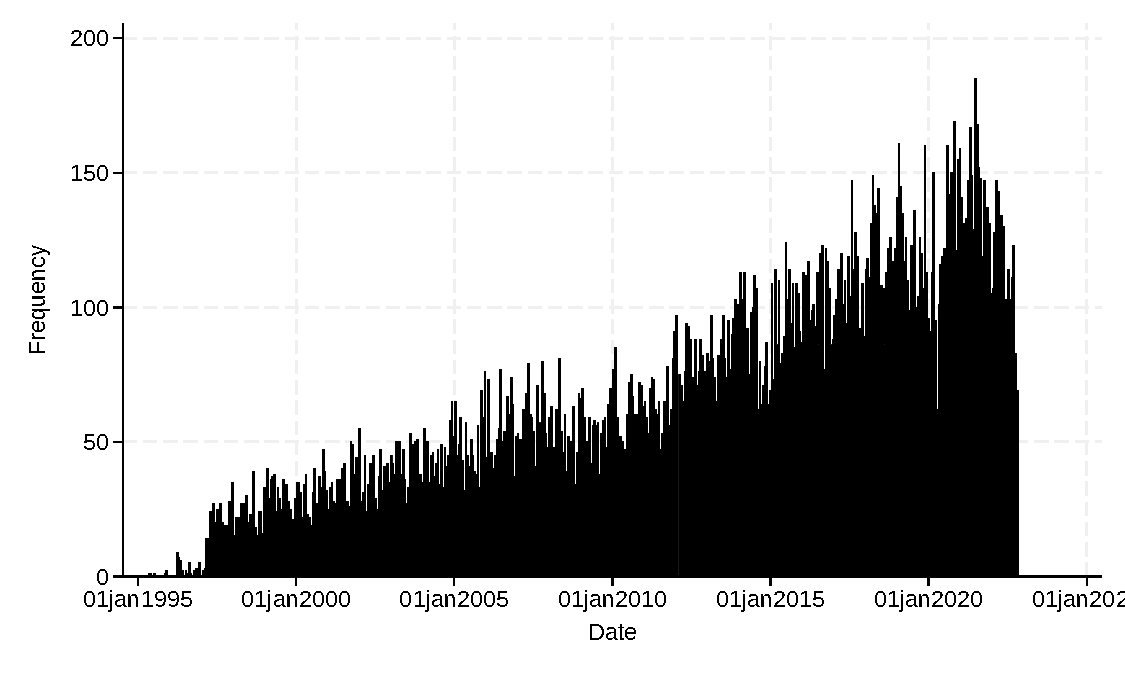
\includegraphics[width=0.8\textwidth]{HA_log/16.pdf}
\end{figure}
\begin{figure}[h!]
    \centering
    \caption{MI episode end dates}
    \label{MIenhist}
    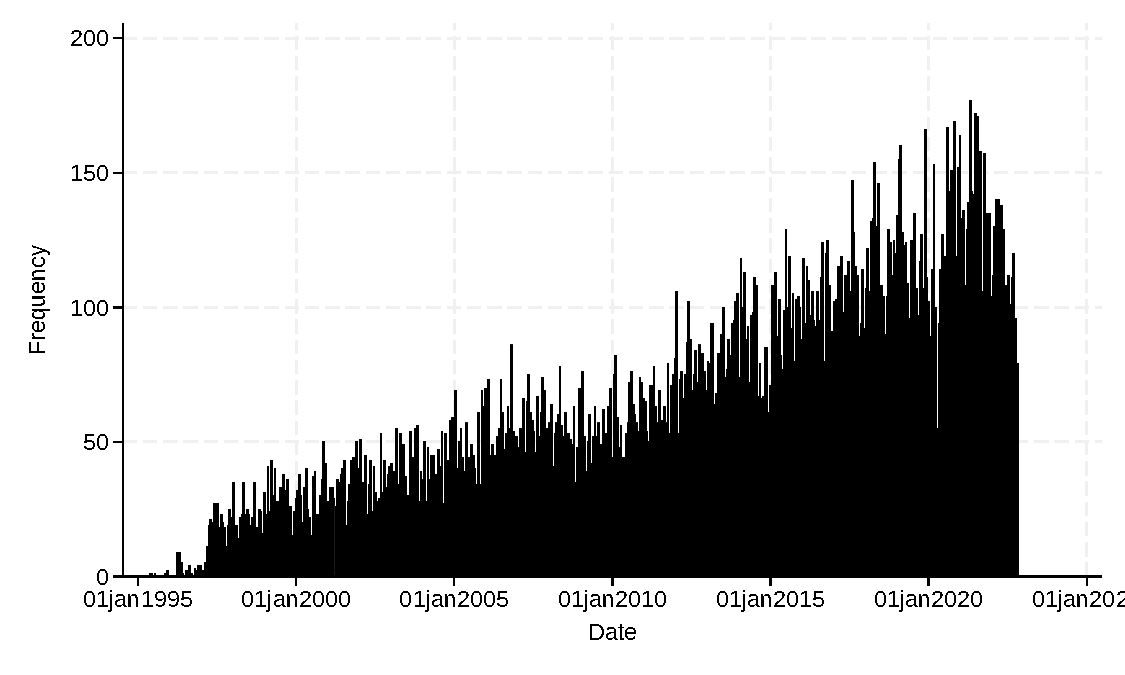
\includegraphics[width=0.8\textwidth]{HA_log/16_1.pdf}
\end{figure}
\begin{figure}[h!]
    \centering
    \caption{All episode start dates}
    \label{sthist}
    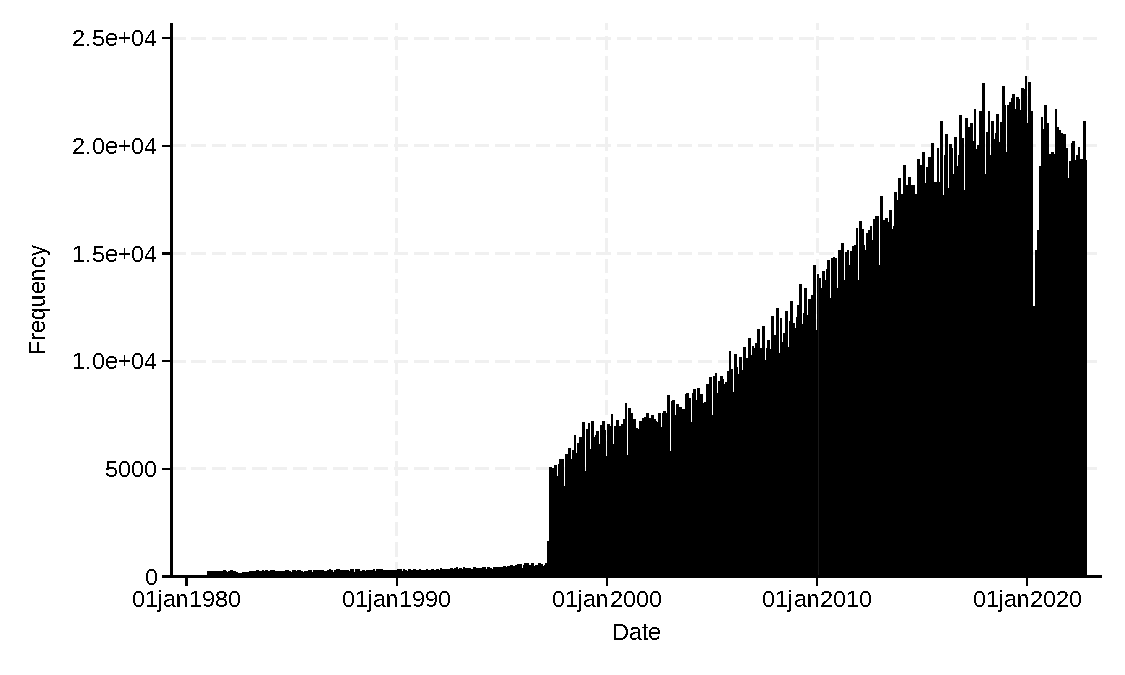
\includegraphics[width=0.8\textwidth]{HA_log/16_2.pdf}
\end{figure}
\begin{figure}[h!]
    \centering
    \caption{All episode end dates}
    \label{enhist}
    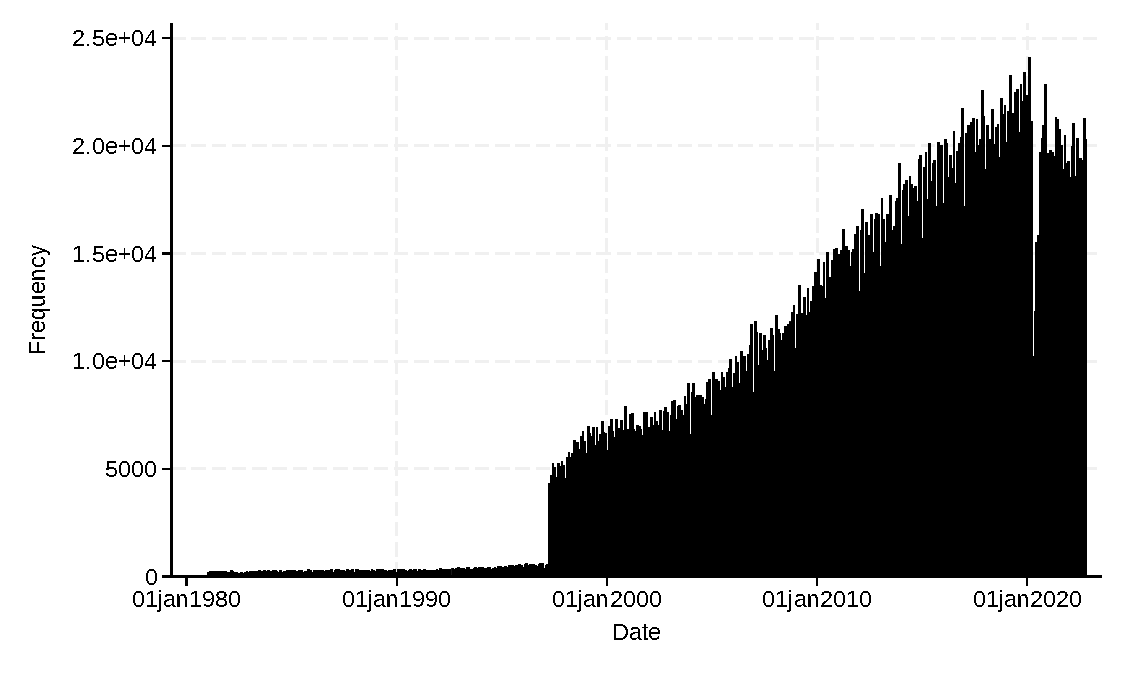
\includegraphics[width=0.8\textwidth]{HA_log/16_3.pdf}
\end{figure}
\begin{stlog}. gen epist = date(epistart,"DMY")
(57,149 missing values generated)
{\smallskip}
. gen epien = date(epiend,"DMY")
(57,446 missing values generated)
{\smallskip}
. format epist epien \%td
{\smallskip}
. *Check missing values and replace with admission and discharge dates if necesary
. count if epist==.
  57,149
{\smallskip}
. count if epist==. \& admidate==""
  42
{\smallskip}
. replace epist = date(admidate,"DMY") if epist==.
(57,107 real changes made)
{\smallskip}
. drop if epist==.
(42 observations deleted)
{\smallskip}
. count if epien==.
  57,404
{\smallskip}
. count if epien==. \& disdate==""
  314
{\smallskip}
. replace epien = date(disdate,"DMY") if epien==.
(57,090 real changes made)
{\smallskip}
. replace epien = epist if epien==.
(314 real changes made)
{\smallskip}
. *Check distributions
. hist epist if MI == 1, color(black) graphregion(color(white)) ///
> frequency xtitle("Date") bin(500)
(bin=500, start=12906, width=20.086)
{\smallskip}
. hist epien if MI == 1, color(black) graphregion(color(white)) ///
> frequency xtitle("Date") bin(500)
(bin=500, start=12912, width=20.074)
{\smallskip}
. hist epist, color(black) graphregion(color(white)) ///
> frequency xtitle("Date") bin(500)
(bin=500, start=7641, width=30.616)
{\smallskip}
. hist epien, color(black) graphregion(color(white)) ///
> frequency xtitle("Date") bin(500)
(bin=500, start=7671, width=30.556)
{\smallskip}
. gen admmode = 1
{\smallskip}
. replace admmode = 0 if inrange(admisorc,1000,2002) | inrange(admisorc,4000,4001) ///
>  | inrange(admisorc,7000,7003) | (admisorc >= 10000 \& admisorc!=11000)
(4,046,768 real changes made)
{\smallskip}
. ta admmode
{\smallskip}
    admmode {\VBAR}      Freq.     Percent        Cum.
\HLI{12}{\PLUS}\HLI{35}
          0 {\VBAR}  4,046,768       96.91       96.91
          1 {\VBAR}    129,168        3.09      100.00
\HLI{12}{\PLUS}\HLI{35}
      Total {\VBAR}  4,175,936      100.00
{\smallskip}
. *The vast majority are from home
. gen sepmode = 1
{\smallskip}
. replace sepmode = 0 if inrange(disdest,1000,2002) | inrange(disdest,4000,4001) ///
>  | inrange(disdest,7000,7003) | (disdest >= 10000 \& disdest!=11000)
(3,765,066 real changes made)
{\smallskip}
. replace sepmode = 2 if disdest==11001
(19,565 real changes made)
{\smallskip}
. ta sepmode
{\smallskip}
    sepmode {\VBAR}      Freq.     Percent        Cum.
\HLI{12}{\PLUS}\HLI{35}
          0 {\VBAR}  3,745,501       89.69       89.69
          1 {\VBAR}    410,870        9.84       99.53
          2 {\VBAR}     19,565        0.47      100.00
\HLI{12}{\PLUS}\HLI{35}
      Total {\VBAR}  4,175,936      100.00
{\smallskip}
. *Again, the vast majority discharge home
\end{stlog}
\color{black}

Any dates you use should be checked. Visualisation is the simplest way to do this. 
What you're looking for is potential errors and to understand the shape of the data. 
For example, in Figure~\ref{MIsthist}, we see a `jump' in MI admissions around 1997 --
likely inidicating one or more datasets begins here (or earlier data
was coded using ICD-9, or any other reason). We also see that the data falls off
around 2022. We also note the seasonality of MI admissions and can see a
dip in admissions around the time COVID-19 lockdowns started (becoming much more 
noticeable when including all admissions; Figure~\ref{sthist}). 

Also note there's a ``problem'' with the output of the admission source and discharge destination
codes -- within a given healthcare system, you would expect the number of episodes coded as 
having transferred on discharge should approximate the number of episodes coded as being admitted from a 
transfer (because they're transferring within a healthcare system). This is clearly not the case,
meaning one of these fields is not ``correctly'' coded (correctly for our purposes, 
there may be a genuine reason these don't align). Just something to keep in mind
when doing further processing. 

\clearpage
\subsection{Finding and removing ``duplicate'' and ``nested'' admissions}

As above, we first remove admissions on the same day as the previous admissions, 
but keep the relevant information they contain. In doing so, we're making the assumption
that two admissions on the same day for MI are related to a single event,
and not two separate MI's. This seems like a reasonable assumption. 

Then, the same for nested admissions. Note that both admission and separation date
are updated in each iteration. 

Both processes will be looped to capture individuals with multiple MI admissions. 
The number of loops is determined by running them until no further changes occur. 

\color{Blue4}
\begin{stlog}*Drop same day admissions, but keep the information they contain
forval i = 1/5 {\lbr}
bysort eid (epist epien sepmode) : gen A = 1 if epist == epist[_n-1] \& epien == epien[_n-1]
bysort eid (epist epien sepmode) : replace A =. if A[_n-1]==1
bysort eid (epist epien sepmode) : replace MI = 1 if MI[_n+1]==1 \& A[_n+1]==1
bysort eid (epist epien sepmode) : replace sepmode = sepmode[_n+1] if sepmode[_n+1]!=0 \& A[_n+1]==1
drop if A == 1
drop A
{\rbr}
*Drop nested admissions, but keep the information they contain.
forval i = 1/100 {\lbr}
bysort eid (epist epien sepmode) : gen A = 1 if epist < epien[_n-1] \& epien[_n-1]!=.
bysort eid (epist epien sepmode) : replace A =. if A[_n-1]==1
bysort eid (epist epien sepmode) : replace MI = 1 if MI[_n+1]==1 \& A[_n+1]==1
bysort eid (epist epien sepmode) : replace epist = epist[_n+1] if epist[_n+1] < epist \& A[_n+1]==1
bysort eid (epist epien sepmode) : replace sepmode = sepmode[_n+1] if sepmode[_n+1]==1 \& epien[_n+1]
>  > epien \& A[_n+1]==1
bysort eid (epist epien sepmode) : replace sepmode = sepmode[_n+1] if sepmode[_n+1]==2 \& A[_n+1]==1
bysort eid (epist epien sepmode) : replace epien = epien[_n+1] if epien[_n+1] > epien \& A[_n+1]==1
drop if A == 1
drop A
{\rbr}
\end{stlog}
\color{black}

\clearpage
\subsection{Identifying and removing transfers}

First, it's worth looking at the time between admissions
for potential transfers. 

\color{Blue4}
\begin{figure}[h!]
    \centering
    \caption{Time between admissions.}
    \label{transferhist1}
    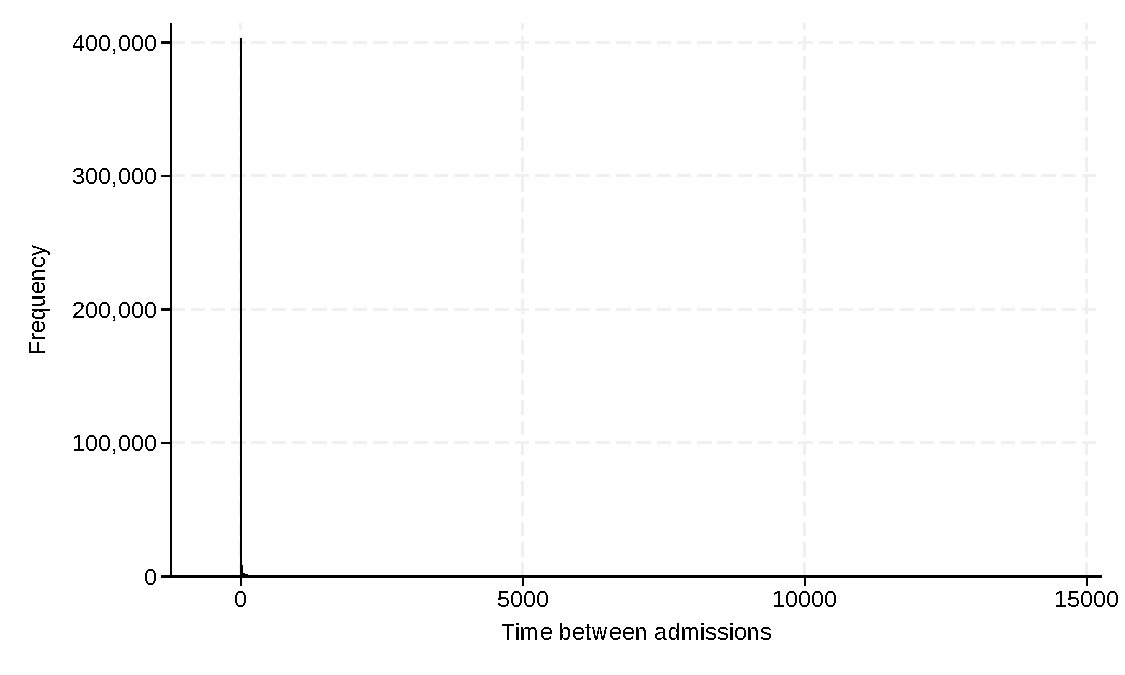
\includegraphics[width=0.8\textwidth]{HA_log/18.pdf}
\end{figure}
\begin{figure}[h!]
    \centering
    \caption{Time between admissions for an MI constrained to values between -30 and 30.}
    \label{transferhist2}
    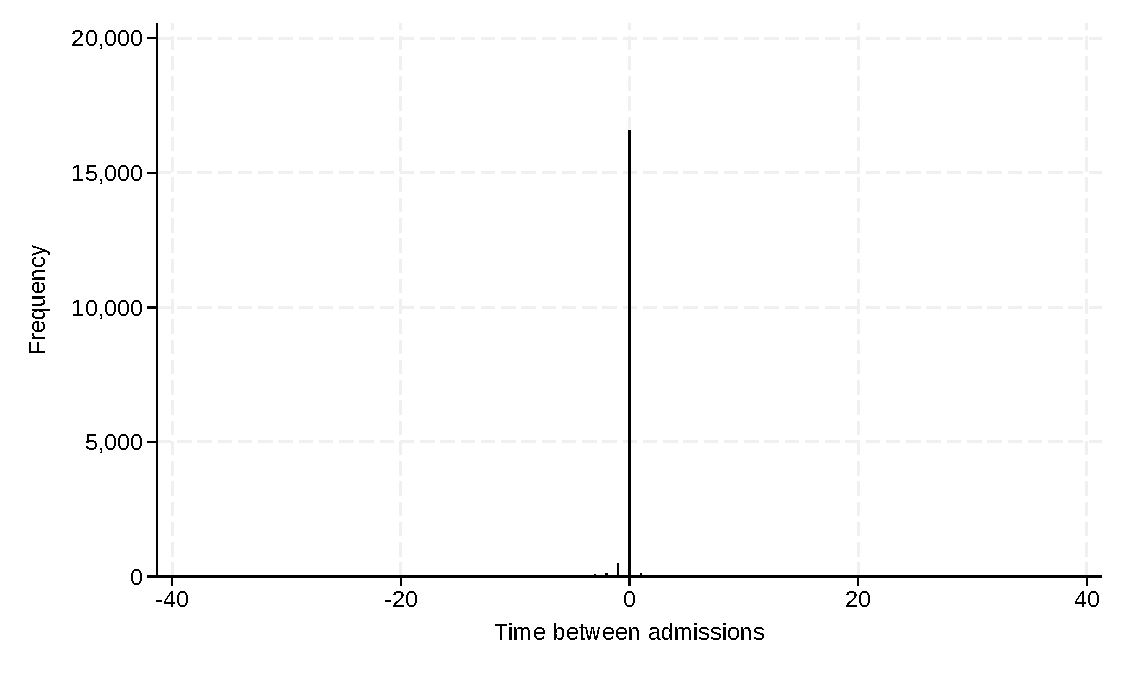
\includegraphics[width=0.8\textwidth]{HA_log/18_1.pdf}
\end{figure}
\begin{figure}[h!]
    \centering
    \caption{Time between admissions for an MI constrained to values between -30 and 30, excluding 0.}
    \label{transferhist3}
    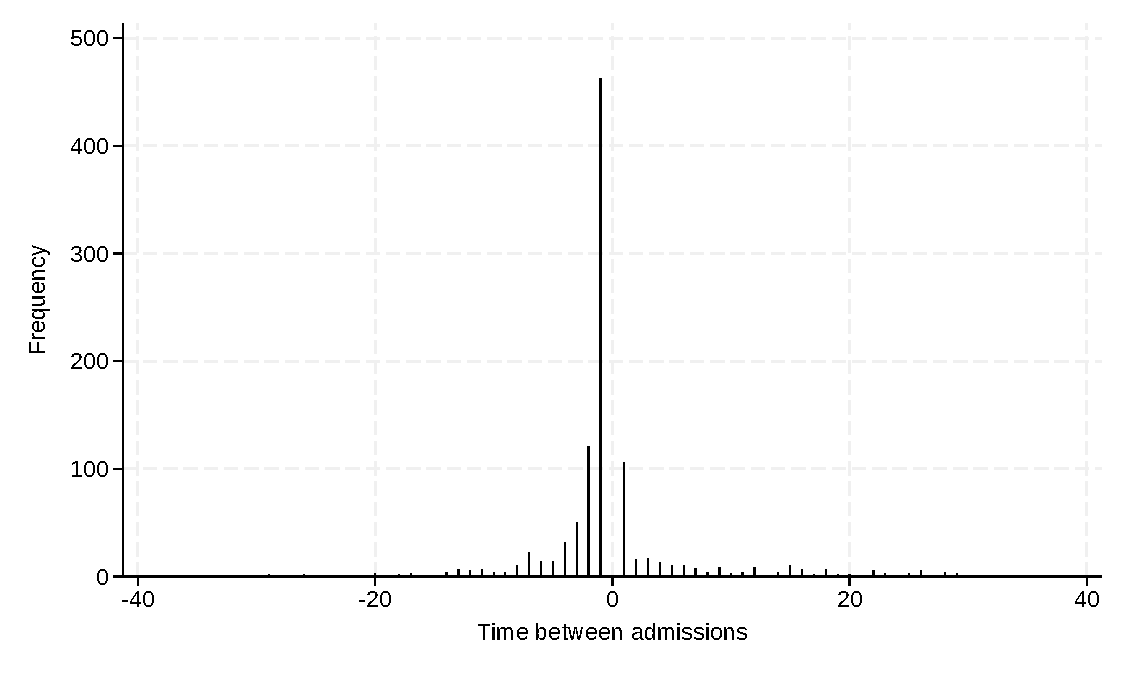
\includegraphics[width=0.8\textwidth]{HA_log/18_2.pdf}
\end{figure}
\begin{stlog}*Tag potential transfers
bysort eid (epist epien sepmode) : gen ptr = 1 if admmode==1 | sepmode[_n-1]==1
*Distance between transfers
bysort eid (epist epien sepmode) : gen transferdist = epist-epien[_n-1]
hist transferdist if ptr == 1, bin(1000) color(gs0) frequency graphregion(color(white)) ///
xtitle("Time between admissions") ylabel(,format(\%9.0fc) angle(0))
hist transferdist if inrange(transferdist,-30,30) \& ///
MI[_n-1]==1 \& ptr == 1, ///
bin(1000) color(gs0) frequency graphregion(color(white)) ///
xtitle("Time between admissions") ylabel(,format(\%9.0fc) angle(0))
hist transferdist if inrange(transferdist,-30,30) \& transferdist!=0 \& ///
MI[_n-1]==1 \& ptr == 1, ///
bin(1000) color(gs0) frequency graphregion(color(white)) ///
xtitle("Time between admissions") ylabel(,format(\%9.0fc) angle(0))
> luding 0.)
\end{stlog}
\color{black}

From these figures (Figures~\ref{transferhist1}-\ref{transferhist13}) we see that most 
transfers occur on the same day, or one day after, the seperation for the 
initial admission. At this point, we have to make a decision
about how long we are going to allow between events. Given that 
it appears that ~16,000 transfer admissions have a transfer date that
matches the previous admission date, compared to just 100 with that distance being
1 day, and even fewer with 2, 3, etc., it doesn't really matter if we set a ``buffer''
(i.e., a period of time where we assume that a transfer did occur even if the
dates don't match perfectly or that we are missing data). Thus, here, we will assume the data coding is not perfect, 
and if someone has transferred within 1 day, we will assume that it is indeed a transfer, 
and not a new admission. 

Moreover, if the next episode of care occurs on the exact same day as the original
admission, we are going to assume it is more likely that 
this is an admission where the transfer has been mis-coded (or gain, that we have missing data)
than it is a new admission.

\color{Blue4}
\begin{stlog}gen tr = 1 if ptr == 1 \& inrange(transferdist,0,1)
bysort eid (epist epien sepmode) : replace tr = 1 if transferdist==0 \& (MI==1 | MI[_n-1]==1)
*Only deal with one at a time
bysort eid (epist epien sepmode) : replace tr =. if tr[_n-1]==1
*Drop transfers, but keep the information they contain
bysort eid (epist epien sepmode) : replace MI = 1 if MI[_n+1]==1 \& tr[_n+1]==1
bysort eid (epist epien sepmode) : replace epien = epien[_n+1] if tr[_n+1]==1
bysort eid (epist epien sepmode) : drop if tr == 1 \& tr[_n-1]==.
drop ptr tr transferdist
*This introduces new nested admissions, so we need to cycle between dropping transfers and nested ad
> missions
bysort eid (epist epien sepmode) : gen A = 1 if epist < epien[_n-1] \& epien[_n-1]!=.
bysort eid (epist epien sepmode) : replace A =. if A[_n-1]==1
bysort eid (epist epien sepmode) : replace MI = 1 if MI[_n+1]==1 \& A[_n+1]==1
bysort eid (epist epien sepmode) : replace epist = epist[_n+1] if epist[_n+1] < epist \& A[_n+1]==1
bysort eid (epist epien sepmode) : replace sepmode = sepmode[_n+1] if sepmode[_n+1]==1 \& epien[_n+1]
>  > epien \& A[_n+1]==1
bysort eid (epist epien sepmode) : replace sepmode = sepmode[_n+1] if sepmode[_n+1]==2 \& A[_n+1]==1
bysort eid (epist epien sepmode) : replace epien = epien[_n+1] if epien[_n+1] > epien \& A[_n+1]==1
drop if A == 1
drop A
forval i = 1/100 {\lbr}
bysort eid (epist epien sepmode) : gen ptr = 1 if admmode==1 | sepmode[_n-1]==1
bysort eid (epist epien sepmode) : gen transferdist = epist-epien[_n-1]
gen tr = 1 if ptr == 1 \& inrange(transferdist,0,1)
bysort eid (epist epien sepmode) : replace tr = 1 if transferdist==0 \& (MI==1 | MI[_n-1]==1)
bysort eid (epist epien sepmode) : replace tr =. if tr[_n-1]==1
bysort eid (epist epien sepmode) : replace MI = 1 if MI[_n+1]==1 \& tr[_n+1]==1
bysort eid (epist epien sepmode) : replace epien = epien[_n+1] if tr[_n+1]==1
bysort eid (epist epien sepmode) : drop if tr == 1 \& tr[_n-1]==.
drop ptr tr transferdist
bysort eid (epist epien sepmode) : gen A = 1 if epist < epien[_n-1] \& epien[_n-1]!=.
bysort eid (epist epien sepmode) : replace A =. if A[_n-1]==1
bysort eid (epist epien sepmode) : replace MI = 1 if MI[_n+1]==1 \& A[_n+1]==1
bysort eid (epist epien sepmode) : replace epist = epist[_n+1] if epist[_n+1] < epist \& A[_n+1]==1
bysort eid (epist epien sepmode) : replace sepmode = sepmode[_n+1] if sepmode[_n+1]==1 \& epien[_n+1]
>  > epien \& A[_n+1]==1
bysort eid (epist epien sepmode) : replace sepmode = sepmode[_n+1] if sepmode[_n+1]==2 \& A[_n+1]==1
bysort eid (epist epien sepmode) : replace epien = epien[_n+1] if epien[_n+1] > epien \& A[_n+1]==1
drop if A == 1
drop A
{\rbr}
*And that's it. 
keep if MI == 1
keep eid epist epien MI
save AllMI, replace
\end{stlog}
\color{black}

\clearpage
\subsection{Checking the processed dataset}

As mentioned above, the whole time you are developing this code
you should be carefully watching what it does and seeing if it makes sense. 
But now that it's ``done'', it's also worth doing some final checks to see if we
can detect any final errors. 

First, we check that no events have been dropped completely.

\color{Blue4}
\begin{stlog}use AllMI, clear
collapse (sum) MI, by(eid)
rename MI nMI
save tempcheck, replace
use HESIN, clear
merge 1:m eid ins_index using hesinmi
drop _merge
collapse (sum) MI, by(eid)
merge 1:1 eid using tempcheck
drop _merge
recode nMI .=0
\end{stlog}
\begin{stlog}. count if MI < nMI
  0
{\smallskip}
. count if MI > nMI \& nMI==0
  0
{\smallskip}
. erase tempcheck.dta
{\smallskip}
\end{stlog}
\color{black}

Next, we check there aren't any duplicate events
and that the number of events per person seems reasonable. 

\color{Blue4}
\begin{stlog}. use AllMI, clear
{\smallskip}
. bysort eid epist : gen njm = _n
{\smallskip}
. ta njm
{\smallskip}
        njm {\VBAR}      Freq.     Percent        Cum.
\HLI{12}{\PLUS}\HLI{35}
          1 {\VBAR}     18,289      100.00      100.00
\HLI{12}{\PLUS}\HLI{35}
      Total {\VBAR}     18,289      100.00
{\smallskip}
. bysort eid (epist) : gen nj = _N
{\smallskip}
. ta nj
{\smallskip}
         nj {\VBAR}      Freq.     Percent        Cum.
\HLI{12}{\PLUS}\HLI{35}
          1 {\VBAR}     14,216       77.73       77.73
          2 {\VBAR}      2,794       15.28       93.01
          3 {\VBAR}        783        4.28       97.29
          4 {\VBAR}        304        1.66       98.95
          5 {\VBAR}        105        0.57       99.52
          6 {\VBAR}         54        0.30       99.82
          7 {\VBAR}          7        0.04       99.86
          8 {\VBAR}          8        0.04       99.90
         18 {\VBAR}         18        0.10      100.00
\HLI{12}{\PLUS}\HLI{35}
      Total {\VBAR}     18,289      100.00
{\smallskip}
\end{stlog}
\color{black}

It's possible that there is an error for the individual with 18 MIs,
but it's also entirely possible that someone had 18 MIs during 10 years 
of follow-up. We can't show this, but at this point it's worth examining 
the complete admission history for the individuals with high numbers
of admissions to see if you have missed anything obvious, or if the result
is reasonable. In our case, it does indeed look like an individual with 18 MIs. 

Finally, we check the overall dataset.

\color{Blue4}
\begin{figure}[h!]
    \centering
    \caption{Histogram of date of admission for MI.}
    \label{epistMIhist1}
    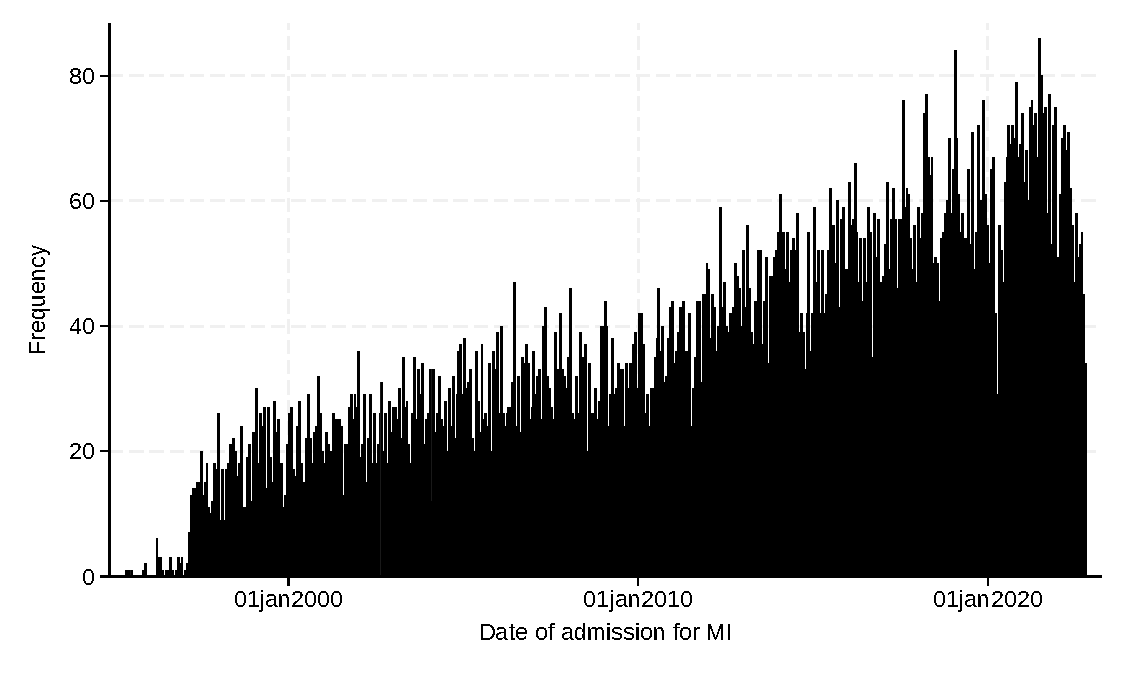
\includegraphics[width=0.8\textwidth]{HA_log/23.pdf}
\end{figure}
\begin{figure}[h!]
    \centering
    \caption{Histogram of date of discharge following MI.}
    \label{epienMIhist1}
    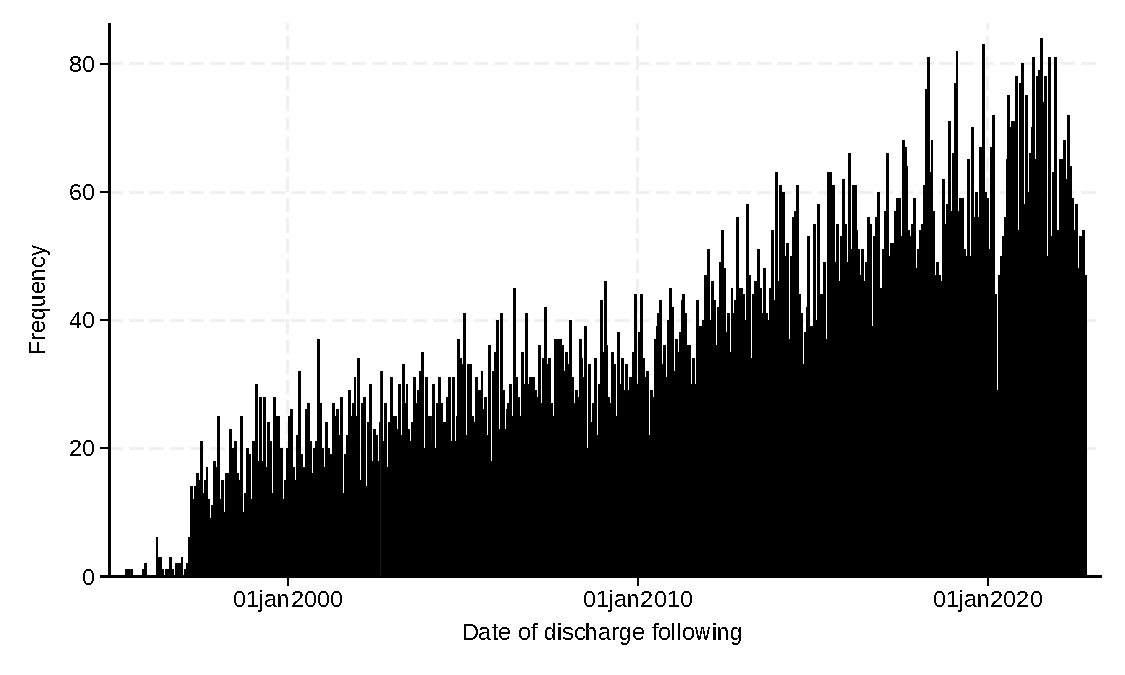
\includegraphics[width=0.8\textwidth]{HA_log/23_1.pdf}
\end{figure}
\begin{figure}[h!]
    \centering
    \caption{Histogram of length of stay for an MI.}
    \label{LOSMIhist1}
    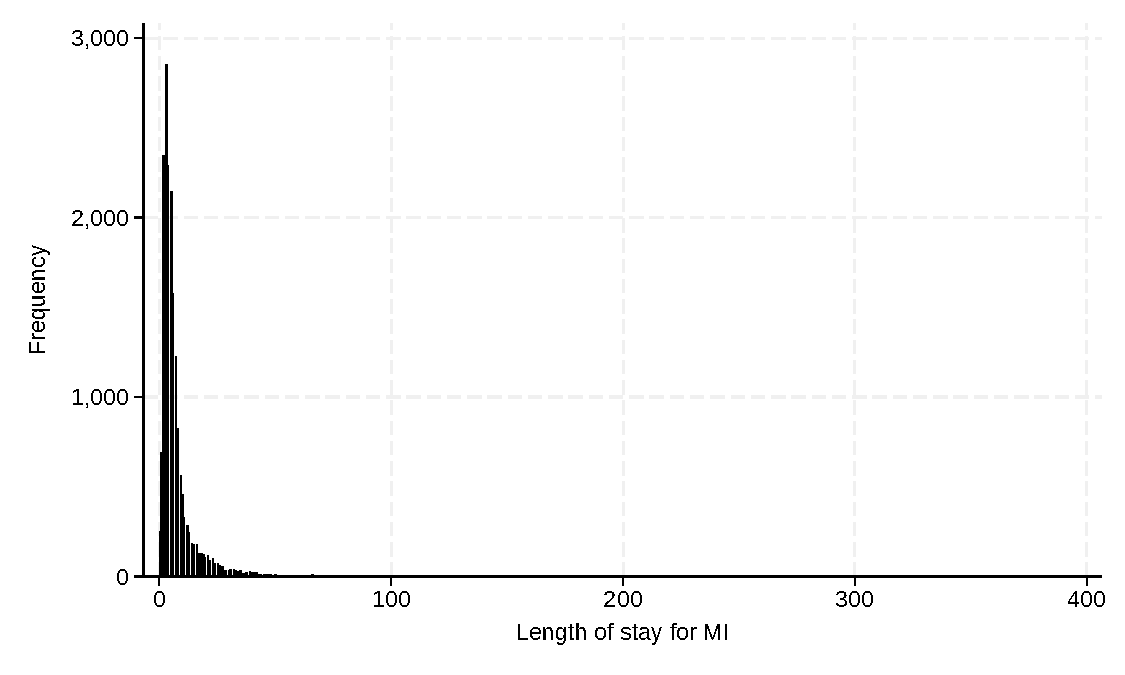
\includegraphics[width=0.8\textwidth]{HA_log/23_2.pdf}
\end{figure}
\begin{stlog}. use AllMI, clear
{\smallskip}
. hist epist, bin(500) color(gs0) frequency graphregion(color(white)) ///
> xtitle("Date of admission for MI") ylabel(,format(\%9.0fc) angle(0)) ///
> tlabel(01jan2000 01jan2010 01jan2020)
(bin=500, start=12906, width=20.084)
{\smallskip}
. hist epien, bin(500) color(gs0) frequency graphregion(color(white)) ///
> xtitle("Date of discharge following `i'") ylabel(,format(\%9.0fc) angle(0)) ///
> tlabel(01jan2000 01jan2010 01jan2020)
(bin=500, start=12912, width=20.074)
{\smallskip}
. gen LOS = epien-epist
{\smallskip}
. count if LOS < 0
  0
{\smallskip}
. hist LOS, bin(500) color(gs0) frequency graphregion(color(white)) ///
> xtitle("Length of stay for MI") ylabel(,format(\%9.0fc) angle(0))
(bin=500, start=0, width=.692)
{\smallskip}
. su LOS, detail
{\smallskip}
                             LOS
\HLI{61}
      Percentiles      Smallest
 1\%            0              0
 5\%            1              0
10\%            2              0       Obs              18,289
25\%            3              0       Sum of wgt.      18,289
{\smallskip}
50\%            5                      Mean           7.640932
                        Largest       Std. dev.      11.13823
75\%            8            242
90\%           16            247       Variance       124.0602
95\%           23            265       Skewness       8.785268
99\%           48            346       Kurtosis       147.2561
{\smallskip}
\end{stlog}
\color{black}

These 0-day MIs seem like an error, but after manually checking a few
of them in the unprocessed dataset, they appear to be ``real''. 

\subsection{Effects of processing data}

So, we just spent a long time doing a lot of data processing. 
Many people just analyse admissions as an outcome in themselves, 
so it's worth emphasising why you would perform data processing like this. 
One situtation where I can think of why you wouldn't do this would be analysing time
to first event, where the only date of relevance is the episode start date. 
In most other situations when analysing events or episodes of care, 
including studying anything to do with what happens
after an event, most of the data processing outlined above is necessary. 

Let's take a look at how necessary it really is.

\color{Blue4}
\begin{stlog}. use hesinmi, clear
{\smallskip}
. count if MI == 1
  33,170
{\smallskip}
. local A = r(N)
{\smallskip}
. use AllMI, clear
{\smallskip}
. count if MI == 1
  18,289
{\smallskip}
. di round(100-100*r(N)/`A',1)
45
{\smallskip}
\end{stlog}
\color{black}

Clearly necessary in our case -- the difference between the unprocessed and processed data
is almost double (i.e., any analysis that didn't involve data processing would
overestimate the rate of MI almost two-fold). This effect of overcounting
has been previously shown in Australian linked data \color{blue}
\href{https://bmjopen.bmj.com/content/7/11/e019226}{Lopez et al., BMJ Open, 2017}\color{black}).


Now it's worth checking this for 
a few other outcomes to emphasise how variable the effects of data processing are.
We will repeat the data processing for the following primary admission diagnoses (ICD-10 codes):
\begin{itemize}
\item Lung cancer (C34)
\item Heart failure (I50)
\item Stroke (I60-I64)
\item Pneumonia (J44)
\item Acute Kidney Failure (N17)
\item Head injury (S00-S09)
\end{itemize}

Notice here we skip the data checking steps and just include the same rules as for MI
 -- this is for brevity in this document only, don't do this for real studies. 

\color{Blue4}
\begin{stlog}foreach oc in LC HF ST PN AK HI {\lbr}
use HESIN_DIAG, clear
keep if level == 1
if "`oc'" == "LC" {\lbr}
gen OC = 1 if substr(diag,1,3)=="C34"
{\rbr}
if "`oc'" == "HF" {\lbr}
gen OC = 1 if substr(diag,1,3)=="I50"
{\rbr}
if "`oc'" == "ST" {\lbr}
gen OC = 1 if inrange(diag,"I60","I649")
{\rbr}
if "`oc'" == "PN" {\lbr}
gen OC = 1 if substr(diag,1,3)=="J44"
{\rbr}
if "`oc'" == "AK" {\lbr}
gen OC = 1 if substr(diag,1,3)=="N17"
{\rbr}
if "`oc'" == "HI" {\lbr}
gen OC = 1 if inrange(diag,"S00","S099")
{\rbr}
keep if OC == 1
save hesin`oc', replace
use HESIN, clear
merge 1:m eid ins_index using hesin`oc'
gen epist = date(epistart,"DMY")
gen epien = date(epiend,"DMY")
format epist epien \%td
count if epist==.
count if epist==. \& admidate==""
replace epist = date(admidate,"DMY") if epist==.
drop if epist==.
count if epien==.
count if epien==. \& disdate==""
replace epien = date(disdate,"DMY") if epien==.
replace epien = epist if epien==.
gen admmode = 1
replace admmode = 0 if inrange(admisorc,1000,2002) | inrange(admisorc,4000,4001) ///
 | inrange(admisorc,7000,7003) | (admisorc >= 10000 \& admisorc!=11000)
gen sepmode = 1
replace sepmode = 0 if inrange(disdest,1000,2002) | inrange(disdest,4000,4001) ///
 | inrange(disdest,7000,7003) | (disdest >= 10000 \& disdest!=11000)
replace sepmode = 2 if disdest==11001
forval i = 1/5 {\lbr}
bysort eid (epist epien sepmode) : gen A = 1 if epist == epist[_n-1] \& epien == epien[_n-1]
bysort eid (epist epien sepmode) : replace A =. if A[_n-1]==1
bysort eid (epist epien sepmode) : replace OC = 1 if OC[_n+1]==1 \& A[_n+1]==1
bysort eid (epist epien sepmode) : replace sepmode = sepmode[_n+1] if sepmode[_n+1]!=0 \& A[_n+1]==1
drop if A == 1
drop A
{\rbr}
forval i = 1/100 {\lbr}
bysort eid (epist epien sepmode) : gen A = 1 if epist < epien[_n-1] \& epien[_n-1]!=.
bysort eid (epist epien sepmode) : replace A =. if A[_n-1]==1
bysort eid (epist epien sepmode) : replace OC = 1 if OC[_n+1]==1 \& A[_n+1]==1
bysort eid (epist epien sepmode) : replace epist = epist[_n+1] if epist[_n+1] < epist \& A[_n+1]==1
bysort eid (epist epien sepmode) : replace sepmode = sepmode[_n+1] if sepmode[_n+1]==1 \& epien[_n+1]
>  > epien \& A[_n+1]==1
bysort eid (epist epien sepmode) : replace sepmode = sepmode[_n+1] if sepmode[_n+1]==2 \& A[_n+1]==1
bysort eid (epist epien sepmode) : replace epien = epien[_n+1] if epien[_n+1] > epien \& A[_n+1]==1
drop if A == 1
drop A
{\rbr}
bysort eid (epist epien sepmode) : gen ptr = 1 if admmode==1 | sepmode[_n-1]==1
bysort eid (epist epien sepmode) : gen transferdist = epist-epien[_n-1]
gen tr = 1 if ptr == 1 \& inrange(transferdist,0,1)
bysort eid (epist epien sepmode) : replace tr = 1 if transferdist==0 \& (OC==1 | OC[_n-1]==1)
bysort eid (epist epien sepmode) : replace tr =. if tr[_n-1]==1
bysort eid (epist epien sepmode) : replace OC = 1 if OC[_n+1]==1 \& tr[_n+1]==1
bysort eid (epist epien sepmode) : replace epien = epien[_n+1] if tr[_n+1]==1
bysort eid (epist epien sepmode) : drop if tr == 1 \& tr[_n-1]==.
drop ptr tr transferdist
bysort eid (epist epien sepmode) : gen A = 1 if epist < epien[_n-1] \& epien[_n-1]!=.
bysort eid (epist epien sepmode) : replace A =. if A[_n-1]==1
bysort eid (epist epien sepmode) : replace OC = 1 if OC[_n+1]==1 \& A[_n+1]==1
bysort eid (epist epien sepmode) : replace epist = epist[_n+1] if epist[_n+1] < epist \& A[_n+1]==1
bysort eid (epist epien sepmode) : replace sepmode = sepmode[_n+1] if sepmode[_n+1]==1 \& epien[_n+1]
>  > epien \& A[_n+1]==1
bysort eid (epist epien sepmode) : replace sepmode = sepmode[_n+1] if sepmode[_n+1]==2 \& A[_n+1]==1
bysort eid (epist epien sepmode) : replace epien = epien[_n+1] if epien[_n+1] > epien \& A[_n+1]==1
drop if A == 1
drop A
forval i = 1/100 {\lbr}
bysort eid (epist epien sepmode) : gen ptr = 1 if admmode==1 | sepmode[_n-1]==1
bysort eid (epist epien sepmode) : gen transferdist = epist-epien[_n-1]
gen tr = 1 if ptr == 1 \& inrange(transferdist,0,1)
bysort eid (epist epien sepmode) : replace tr = 1 if transferdist==0 \& (OC==1 | OC[_n-1]==1)
bysort eid (epist epien sepmode) : replace tr =. if tr[_n-1]==1
bysort eid (epist epien sepmode) : replace OC = 1 if OC[_n+1]==1 \& tr[_n+1]==1
bysort eid (epist epien sepmode) : replace epien = epien[_n+1] if tr[_n+1]==1
bysort eid (epist epien sepmode) : drop if tr == 1 \& tr[_n-1]==.
drop ptr tr transferdist
bysort eid (epist epien sepmode) : gen A = 1 if epist < epien[_n-1] \& epien[_n-1]!=.
bysort eid (epist epien sepmode) : replace A =. if A[_n-1]==1
bysort eid (epist epien sepmode) : replace OC = 1 if OC[_n+1]==1 \& A[_n+1]==1
bysort eid (epist epien sepmode) : replace epist = epist[_n+1] if epist[_n+1] < epist \& A[_n+1]==1
bysort eid (epist epien sepmode) : replace sepmode = sepmode[_n+1] if sepmode[_n+1]==1 \& epien[_n+1]
>  > epien \& A[_n+1]==1
bysort eid (epist epien sepmode) : replace sepmode = sepmode[_n+1] if sepmode[_n+1]==2 \& A[_n+1]==1
bysort eid (epist epien sepmode) : replace epien = epien[_n+1] if epien[_n+1] > epien \& A[_n+1]==1
drop if A == 1
drop A
{\rbr}
keep if OC == 1
keep eid epist epien OC
save All`oc', replace
{\rbr}
\end{stlog}
\begin{stlog}. foreach oc in LC HF ST PN AK HI {\lbr}
  2. di "`oc'"
  3. use hesin`oc', clear
  4. count if OC == 1
  5. local A = r(N)
  6. use All`oc', clear
  7. count if OC == 1
  8. di round(100-100*r(N)/`A',1)
  9. {\rbr}
LC
  29,274
  26,389
10
HF
  16,486
  9,509
42
ST
  30,569
  16,233
47
PN
  21,029
  12,334
41
AK
  9,866
  5,773
41
HI
  21,957
  17,736
19
{\smallskip}
\end{stlog}
\color{black}

In summary, process your data. 

\end{document}
